\chapter{Grupos}

\section{Conceitos básicos}

\subsection{Grupo e subgrupo}

\begin{definition}
Um \emph{grupo} é uma quádrupla $\bm G=(G,\times,\div,1)$ em que $G$ é um conjunto, $\times \colon G \times G \to G$ é uma operação binária associativa, $1 \in G$ é a identidade com respeito a $\times$ e $\div \colon G \to G$ é a operação unária inversa com respeito a $\times$ e $1$; isto é, $\times$, $1$ e $\div$ satisfazem
	\begin{enumerate}[label=\textbf{G\arabic*.},ref={G\arabic*}]
	\item \label{G1}(Associatividade) Para todos $g_1,g_2,g_3 \in G$,
		\begin{equation*}
		(g_1 \times g_2) \times g_3 = g_1 \times (g_2 \times g_3);
		\end{equation*}
	\item \label{G2} (Identidade) Para todo $g \in G$,
		\begin{equation*}
		1 \times g = g =g \times 1;
		\end{equation*}
	\item \label{G3} (Invertibilidade) Para todo $g \in G$,
		\begin{equation*}
		(\div g) \times g = 1 = g \times (\div g).
		\end{equation*}
	\end{enumerate}
\noindent
Um grupo \emph{comutativo} é um grupo cuja operação binária $\times$ é comutativa; isto é, satisfaz
	\begin{enumerate}[label=\textbf{G\arabic*.},ref={G\arabic*}]
	\setcounter{enumi}{3}
	\item \label{G4} (Comutatividade) Para todos $g_1,g_2 \in G$,
	\begin{equation*}
	g_1 \times g_2 = g_2 \times g_1.
	\end{equation*}
	\end{enumerate}
\end{definition}

\begin{notation}
Denotam-se $g_1g_2 := g_1 \times g_2$ e $g\inv := \div g$ por simplicidade. Quando o grupo é comutativo, em geral denotam-se a operação binária por $+$, a operação unária por $-$ e a constante por $0$, de modo que o grupo é $(G,+,-,0)$.
\end{notation}

O uso do símbolo `$\div$' para representar a função inversa de $\times$ não é usual, mas termos um símbolo para denotar essa função é bastante útil e uma barra como sinal de divisão é bastante comum. Pode-se pensar que, assim como o símbolo `$\times$' é o símbolo `$+$' rotacionado um oitavo de volta, o símbolo `$\div$' é o símbolo `$-$' rotacionado do mesmo tanto.

Em vista das definições introdutórias do capítulo anterior, um grupo é um monoide $\bm G=(G, \times)$ cujos elementos têm inverso sob $\times$ e um grupo comutativo é um grupo cuja operação binária $\times$ é comutativa.

\begin{definition}
Sejam $\bm G = (G,\times,\div,1)$ um grupo, $g \in G$ e $n \in \N$. Definimos
	\begin{equation*}
	g^n := \bigtimes_{i=1}^n g \text{\ \ e\ \ } g^{-n} := \bigtimes_{i=1}^n g^{-1}.
	\end{equation*}
\end{definition}

\begin{proposition}[Leis de corte e inversão]
	Seja $\bm G$ um grupo. Então
	\begin{enumerate}
	\item Para todos $g,g_1,g_2 \in G$ 
		\begin{align*}
		gg_1 = gg_2 &\entao g_1 = g_2 \\
		g_1g = g_2g &\entao g_1 = g_2;
		\end{align*}
	\item Para todos $g_1,\ldots,g_n \in G$, $(g_1 \cdots g_n)^{-1}=g_n^{-1} \cdots g_1^{-1}$.
	\end{enumerate}
\end{proposition}
\begin{proof}
	Se $g g_1 = g g_2$, então
	\begin{equation*}
	g_1 = (g^{-1}g)g_1 = g^{-1}(gg_1) = g^{-1}(gg_2) = (g^{-1}g)g_2 = g_2.
	\end{equation*}
A demonstração da segunda implicação é análoga.
\end{proof}

\begin{definition}
Seja $\bm G = (G,\times,\div,1)$ um grupo. Um \emph{subgrupo} de $\bm G$ é um grupo $\bm S=(S,\times_S,\div_S,1_S)$ em que $S \subseteq G$, $\times_S=\times|_{S \times S}$, $\div = \div|_S$ e $1_S=1$. Denota-se $\bm S \leq \bm G$.

Um subgrupo \emph{próprio} de $\bm G$ é um subgrupo $\bm S \leq \bm G$ tal que $S$ é um conjunto próprio de $G$ ($S  \subset G$). Denota-se $\bm S < \bm G$.
\end{definition}

\begin{proposition}
\label{alge:prop.subgru}
Sejam $\bm G$ um grupo e $S \subseteq G$ que satisfaz
	\begin{enumerate}[label=\textbf{SG\arabic*.},ref={SG\arabic*}]
	\item \label{SG1} (Não-vacuidade) $S \neq \emptyset$;
	\item \label{SG2} (Fechamento) Para todos $s_1,s_2 \in S$, $s_1s_2 \in S$;
	\item \label{SG3} (Invertibilidade) Para todo $s \in S$,  $s\inv \in S$.
	\end{enumerate}	
\noindent
Então $\bm S=(S,\times|_{S \times S}, \div|_S,1)$ é um grupo. Ainda, se $\bm G$ é comutativo, então $\bm S$ é comutativo.
\end{proposition}
\begin{proof}
Por simplicidade, definamos $\star := \times|_{S \times S}$.

%($\Rightarrow$) (\ref{SG1}) Como $\bm S$ é um grupo, $e \in S$, portanto $S \neq \emptyset$.
%(\ref{SG2}) Como $\bm S$ é grupo, $\star$ é uma operação binária, portanto segue que, para todo $s_1,s_2 \in S$, $s_1s_2 \in S$ (\ref{prop:restri.op.bin}).
%(\ref{SG3}) Seja $s \in S$. Como $\bm S$ é grupo, existe $s^{-1} \in S$ inverso de $s$ em $\bm S$. Como $s^ {-1} \in G$, segue da unicidade do inverso que $s^{-1}$ é o inverso de $s$ em $\bm G$.

%($\Leftarrow$)
(Operação binária) Pela primeira e segunda propriedades de $S$, segue que $\star$ é uma operação binária (\ref{prop:restri.op.bin}).\\
(\ref{G1}) Sejam $s_1,s_2,s_3 \in S$. Então
	\begin{equation*}
	(s_1 \star s_2) \star s_3 = (s_1 \times s_2) \times s_3 = s_1 \times (s_2 \times s_3) = s_1 \star (s_2 \star s_3).
	\end{equation*}
(\ref{G2}) Como $S \neq \emptyset$, existe $s \in S$, portanto $s\inv \in S$. Isso implica que $1=s \times s\inv \in S$ e, como $1$ é identidade de $\bm G$, segue que, para todo $s \in S$,
	\begin{equation*}
	1 \star s = 1 \times s = s = s \times 1 = s \star 1.
	\end{equation*}
(\ref{G3}) Seja $s \in S$. Pela terceira propriedade de $S$, segue que o inverso de $s$ em $\bm G$ pertence a $S$. Então
	\begin{equation*}
	s\inv \star s = s\inv \times s = e = s \times s\inv = s \star s\inv,
	\end{equation*}
portanto $s\inv$ é o inverso de $s$ em $\bm S$.

(\ref{G4}) Por fim, suponhamos que $\bm G$ é um grupo comutativo. Sejam $s_1,s_2 \in S$. Como $\times$ é comutativa, então
	\begin{equation*}
	s_1 \star s_2 = s_1 \times s_2 = s_2 \times s_1 = s_2 \star s_1.
	\end{equation*}
\end{proof}

\begin{proposition}
Sejam $\bm G$ um grupo e $\mathcal G$ o conjunto dos subgrupos de $\bm G$. Então $(\mathcal G,\leq)$ é um conjunto parcialmente ordenado.
\end{proposition}
\begin{proof}
Claramente, $\bm G \in \mathcal G$, portanto $\mathcal G$ não é vazio. Mostremos que $\leq$ é uma ordem parcial em $\mathcal G$. (Reflexividade) Seja $\bm S \in \mathcal G$. Então $\bm S \leq \bm S$, pois $\bm S$ é um grupo, $S \subseteq S$ e $\times|_{S \times S} = \times|_{S \times S}$. (Antissimetria) Sejam $\bm{S_1},\bm{S_2} \in \mathcal G$ tais que $\bm{S_1} \leq \bm{S_2}$ e $\bm{S_2} \leq \bm{S_1}$. Então $S_1 \subseteq S_2$ e $S_2 \subseteq S_1$, o que implica $S_1=S_2$, e portanto $\times|_{S_1 \times S_1} = \times|_{S_2 \times S_2}$, o que implica $\bm{S_1} = \bm{S_2}$. (Transitividade) Sejam  $\bm{S_1},\bm{S_2},\bm{S_3} \in \mathcal G$ tais que $\bm{S_1} \leq \bm{S_2}$ e $\bm{S_2} \leq \bm{S_3}$. Então $S_1 \subseteq S_2$ e $S_2 \subseteq S_3$, o que implica $S_1 \subseteq S_3$ e, portanto, $\times_{S_1} = \times|_{S_3 \times S_3}$.
\end{proof}

\begin{proposition}
\label{alge:prop.subgru.triv}
Seja $\bm G$ um grupo. Então $\bm{\{1\}}$ e $\bm G$ são subgrupos de $\bm G$.
\end{proposition}

\begin{proposition}
\label{alge:prop.subgru.inter}
Sejam $\bm G$ um grupo, $(\bm S_i)_{i \in I}$ uma família de subgrupos de $\bm G$ e
	\begin{equation*}
	S := \bigcap_{i \in I} S_i.
	\end{equation*}
Então $\bm S$ é um subgrupo de $\bm G$.
\end{proposition}
\begin{proof}
(\ref{SG1}) Para todo $i \in I$, $\bm{S_i}\leq \bm G$, portanto $e \in N_i$. Logo $e \in N$. (\ref{SG2}) Sejam $s_1, s_2 \in S$. Para todo $i \in I$, $s_1,s_2 \in S_i$. Como $\bm{S_i} \leq \bm G$, segue que $s_1s_2 \in S_i$, o que implica que $s_1s_2 \in S$. (\ref{SG3}) Seja $s \in S$. Para todo $i \in I$, $s \in S_i$ e, como $\bm{S_i} \leq \bm{G}$, segue que $s^{-1} \in S_i$, o que implica que $s^{-1} \in S$.
\end{proof}

\begin{proposition}
\label{alge:prop.subgru.uni}
Sejam $\bm G$ um grupo, $(\bm S_i)_{i \in I}$ uma família superiormente dirigida de subgrupos de $\bm G$ (para todos $i_1,i_2 \in I$, existe $i \in I$ tal que $S_{i_1} \subseteq S_i$ e $S_{i_2} \subseteq S_i$) e
	\begin{equation*}
	S := \bigcup_{i \in I} S_i.
	\end{equation*}
Então $\bm S$ é um subgrupo de $\bm G$.
\end{proposition}
\begin{proof}
(Não-vacuidade) Para todo $i \in I$, $\bm{S_i}\leq \bm G$, portanto $e \in N_i$. Logo $e \in N$. (Fechamento) Sejam $s_1,s_2 \in S$. Existem $i_1,i_2 \in I$ tais que $s_1 \in S_{i_1}$ e $s_2 \in S_{i_2}$ e, pela propriedade, existe $i \in I$ tal que $S_{i_1} \subseteq S_{i} \text{\ \ e\ \ } S_{i_2} \subseteq S_{i}$. Então $s_1,s_2 \in S_i$. Como $\bm{S_i} \leq \bm G$, segue que $s_1s_2 \in S_i$, o que implica que $s_1s_2 \in S$. (Invertibilidade) Seja $s \in S$. Existe $i \in I$ tal que $s \in N_i$ e, como $\bm{S_i} \leq \bm G$, segue que $s^{-1} \in S_i$, o que implica que $s^{-1} \in S$.
\end{proof}

A propriedade definida acima é equivalente a dizer que a família $(S_i)_{i \in I}$ é um conjunto dirigido com respeito a $\subseteq$.

\begin{definition}
	Seja $\bm M$ um monoide. O conjunto dos elementos invertíveis de $M$ é denotado por $M^*$.
\end{definition}

%O asterisco não tem a ver com a operação $\times$ do monoide.

\begin{proposition}
Seja $\bm M = (M,\times,1)$ um monoide. Então existe uma operação unária $\div \colon M^* \to M^*$ tal que $\bm{M^*}=(M^*,\times|_{M^* \times M^*},\div,1)$ é um grupo.
\end{proposition}
\begin{proof}
	Sejam $m_1,m_2 \in M^*$. Então existem $m_1^{-1},m_2^{-1} \in M$ tais que
	\begin{equation*}
	m_1m_1^{-1}=1 \text{\ \ e\ \ } m_2m_2^{-1}=1.
	\end{equation*}
Portanto
	\begin{equation*}
	(m_1m_2)(m_2^{-1}m_1^{-1}) = m_1(m_2m_2^{-1})m_1^{-1} = m_1m_1^{-1} = 1,
	\end{equation*}
o que mostra que $m_1m_2 \in M^*$. Ainda, note que $1 \in M^*$, pois $1 \times 1 = 1$. Como $M^*$ é contém a identidade e é fechado sob $\times$, segue que $(M^*,\times,1)$ é um monoide (\ref{alge:prop.submon}). Por fim, $\bm{M^*}$ é um grupo pois, por definição, todo elemento tem inverso e ele é único.
\end{proof}

\begin{definition}
Sejam $\bm G$ um grupo e $g \in G$. A \emph{conjugação} por $g$ é a função
	\begin{align*}
	\func{C_g}{G}{G}{h}{ghg\inv}.
	\end{align*}
A \emph{translação à direita} por $g$ é a função
	\begin{align*}
	\func{D_g}{G}{G}{h}{hg}.
	\end{align*}
A \emph{translação à esquerda} por $g$ é a função
	\begin{align*}
	\func{E_g}{G}{G}{h}{gh}.
	\end{align*}
\end{definition}

\subsection{Coclasses e índice de subgrupo}

\begin{definition}
Sejam $\bm G$ um grupo, $\bm S \leq \bm G$ um subgrupo e $g \in G$. A \emph{coclasse à esquerda} de $\bm S$ em $\bm G$ com \emph{representante} $g$ é o conjunto
	\begin{equation*}
	gS := \{gs:s \in S\}.
	\end{equation*}
A \emph{coclasse à direita} de $\bm S$ em $\bm G$ com \emph{representante} $g$ é o conjunto
	\begin{equation*}
	Sg := \{sg:s \in S\}.
	\end{equation*}
\end{definition}

Coclasses também são conhecidas como classes laterais. As definições de coclasses à esquerda ou à direita são análogas e, por consequência, toda definição ou proposição envolvendo uma das duas tem uma definição ou proposição dual envolvendo a outra. Por esse motivo, durante este capítulo consideraremos sempre coclasses à esquerda.

\begin{proposition}
\label{alge:prop.gru.coclas}
Sejam $\bm G$ um grupos, $\bm S \leq \bm G$ um subgrupo e $g_1g_2 \in G$. Então
	\begin{enumerate}
	\item $g_1(g_2S) = (g_1g_2)S \text{\ \ e\ \ } (Sg_1)g_2 = S(g_1g_2)$
	\item $g_1S=g_2S \Leftrightarrow g_2^{-1}g_1 \in S$ e $Sg_1=Sg_2 \Leftrightarrow g_2^{-1}g_1 \in S$.
	\end{enumerate}
\end{proposition}
\begin{proof}
	\begin{enumerate}
	\item ($\subseteq$) Seja $g \in g_1(g_2S)$. Existem $g' \in g_2S$ tal que $g=g_1g'$ e, portanto, existe $s \in S$ tal que $g'=g_2s$. Mas então, pela associatividade, $g=g_1(g_2s) = (g_1g_2)s$, e segue que $g \in (g_1g_2)S$.
($\supseteq$) Seja $g \in (g_1g_2)S$. Então existe $s \in S$ tal que $g=(g_1g_2)s$ e, da associatividade, segue que $g=g_1(g_2s)$, logo $g \in g_1(g_2S)$. A outra igualdade é análoga.
	
	\item ($\Leftarrow$) Seja $g \in g_1S=g_2S$. Então existem $s,s' \in S$ tais que $g=g_1s=g_2s'$, logo $g_2^{-1}g_1=s's^{-1}$. Como $\bm S$ é subgrupo, segue que $g_2^{-1}g_1=s's^{-1} \in S$.

\noindent
($\Rightarrow$) ($\subseteq$) Se $g_2^{-1}g_1 \in S$, existe $s \in S$ tal que $g_2^{-1}g_1=s$, portanto $g_1=g_2s$, logo $g_1 \in g_2S$. Assim, dado $g \in g_1S$, existe $s' \in S$ tal que $g=g_1s'$. Como $\bm S$ é subgrupo, $ss' \in S$, logo $g=g_2ss' \in g_2S$. ($\supseteq$) Da mesma forma, como $\bm S$ é subgrupo, $g_1^{-1}g_2=(g_2^{-1}g_1)^{-1}=s^{-1} \in S$, o que implica que $g_2=g_1s^{-1} \in g_1S$. Assim, dado $g \in g_2S$, existe $s' \in S$ tal que $g=g_2s'$. Como $\bm S$ é subgrupo, $s^{-1}s' \in S$, logo $g=g_1s^{-1}s' \in g_2S$.
	\end{enumerate}

\end{proof}

Essa proposição nos permite denotar os conjuntos acima simplesmente por $g_1g_2S$ e $Sg_1g_2$, respectivamente.

A proposição a seguir mostra que as cardinalidades das coclasses de um subgrupo são sempre iguais.

\begin{proposition}
Sejam $\bm G$ um grupo, $\bm S \leq \bm G$ um subgrupo e $g_1,g_2 \in G$. Então
	\begin{equation*}
	\card{g_1S}=\card{g_2S}.
	\end{equation*}
\end{proposition}
\begin{proof}
Considere a relação
	\begin{align*}
	\func{f}{g_1S}{g_2S}{g}{g_2g_1\inv g}.
	\end{align*}
Vamos mostrar que $f$ é função; isto é, está bem definida, que $g_1^{-1}g \in S$. Primeiro, note que, se $g \in g_1S$, existe $s\in S$ tal que $g=g_1s$. Então segue que $f(s)=g_2g_1^{-1}g=g_2g_1^{-1}g_1s=g_2s \in g_2S$, o que mostra que $f$ está bem definida. Agora, note que a função
	\begin{align*}
	\func{f\inv}{g_2S}{g_1S}{g}{g_1g_2\inv g},
	\end{align*}
que está bem definida pelo mesmo argumento de cima, é a inversa de $f$, pois $f^{-1} \circ f=1_{g_1S}$ e $f \circ f^{-1}=1_{g_2S}$. Isso mostra que $f$ é uma bijeção. Portanto $\card{g_1S}=\card{g_2S}$.

%Para notar isso, mostraremos que existe bijeção entre $S$ e $gS$.
%	\begin{align*}
%	\func{S}{gS}{s}{gs.}
%	\end{align*}
% Note que a função $f$ é injetiva, pois, se $gs_1=gs_2$, então $s_1=g^{-1}gs_1=g^{-1}gs_2=s_2$.	Agora, note que $f$ é sobrejetiva, pois, se $s' \in gS$, existe $s \in S$ tal que $s'=gs$, logo $f(s)=s'$. Portanto segue que $\card{g_1S} = \card{S}$ e $\card{S} = \card{g_2S}$. Logo $\card{g_1S}=\card{g_2S}$ (\ref{conj:prop.card.rel.equiv}).
\end{proof}

% Poderia chamar essa relação de equivalência de "congruência à esquerda/direita por S", pois a noção de congruência é uma noção algébrica mais geral. No entanto, acho que essa noção de congruência só vale quando podemos quocientar, logo só valeria para subgrupos normais. Poderíamos chamar de "relação de equivalência induzida por S" também.
\begin{proposition}
Sejam $\bm G$ um grupo e $\bm S \leq \bm G$ um subgrupo. A relação binária $\sim$ em $G$ definida por
	\begin{equation*}
	g_1 \sim g_2 \sse g_2^{-1}g_1 \in S
	\end{equation*}
é uma relação de equivalência e suas classes de equivalência são as coclasses à esquerda (à direita) de $\bm S$ em $\bm G$.
\end{proposition}
\begin{proof}
Primeiro vamos demonstrar as três propriedades de relação de equivalência. (Reflexividade) Seja $g \in G$. Então $g^{-1}g=e \in S$, pois $S$ é subgrupo. Logo $g \sim g$. (Simetria) Sejam $g_1,g_2 \in G$. Se $g_2^{-1}g_1 \in S$, como $S$ é subgrupo, então $g_1^{-1}g_2=(g_2^{-1}g_1)^{-1} \in S$. Logo $g_2 \sim g_1$. (Transitividade) Sejam $g_1,g_2,g_3 \in G$. Se $g_1 \sim g_2$ e $g_2 \sim g_3$, então $g_2^{-1}g_1 \in S$ e $g_3^{-1}g_2 \in S$. Como $S$ é subgrupo, segue que $g_3^{-1}g_1=g_3^{-1}g_2g_2^{-1}g_1 \in S$. Logo $g_1 \sim g_3$.

Agora, seja $g \in G$. Vamos mostrar que $[g]=gS$. Seja $s \in [g]$. Então $s \sim g$, o que implica que $g^{-1}s \in S$, que por sua vez implica que existe $s' \in S$ tal que $s'=g^{-1}s$ e, portanto, $s=gs'$. Logo $s \in gS$. Agora, seja $s \in gS$. Então existe $s' \in S$ tal que $s=gs'$, o que implica $g^{-1}s=s'$, que por sua ve implica $g^{-1}s \in S$ e, portanto, $s \sim g$. Logo $s \in [g]$.
\end{proof}

Como $\sim$ é relação de equivalência, particiona $G$, e essas partições são as coclasses de $\bm S$ em $\bm G$. Assim, podemos considerar o conjunto $G/S$ das classes de equivalências como o conjunto das coclasses de $S$ em $\bm G$. É importante notar que esse conjunto ainda não possui estrutura de grupo. Isso será possível mais à frente, mas não para qualquer subgrupo, somente subgrupos que chamamos de normais.

\begin{definition}
Sejam $\bm G$ um grupo e $\bm S \leq \bm G$ um subgrupo. O \emph{conjunto quociente} de $\bm G$ por $\bm S$ é o conjunto
	\begin{equation*}
	G/S := G/\sim.
	\end{equation*}
\end{definition}

\begin{definition}
Seja $\bm G$ um grupo e $\bm S \leq \bm G$ subgrupo. O \emph{índice} de $\bm S$ em $\bm G$ é número cardinal
	\begin{equation*}
	[G : S] := \card{G/S}.
	\end{equation*}
\end{definition}

\begin{proposition}
Sejam $\bm G$ um grupo e $\bm S \leq \bm G$ um subgrupo. Então
	\begin{equation*}
	\card{G}=[G:S] \times \card{S}.
	\end{equation*}
\end{proposition}
\begin{proof}
O conjunto $G/S$ é uma partição de $G$, pois é um conjunto quociente (\ref{conj:teo.rel.equiv.part}). Isso implica que $G/S$ é uma família de conjuntos não vazios, disjuntos dois a dois, e que $G = \bigcup_{[g] \in G/S} gS$. Da terceira condição temos que
	\begin{equation*}
	\card{G} = \card{\bigcup_{[g] \in G/S} gS}.
	\end{equation*}
Da segunda condição, temos por \ref{conj:prop.un.dis} que
	\begin{equation*}
	\card{\bigcup_{[g] \in G/S} gS} = \card{\bigsqcup_{[g] \in G/S} gS}.
	\end{equation*}
Por fim, da primeira condição e do fato de que as coclasses de $S$ têm a mesma cardinalidade, concluímos por \ref{conj:prop.card.un.dis} que
	\begin{equation*}
	\card{\bigsqcup_{[g] \in G/S} gS} = \card{G/S} \times \card{S}.
	\end{equation*}
Disso segue que $\card{G}=[G:S] \times \card{S}$.
\end{proof}

\subsection{Subgrupo normal e grupo quociente}

\begin{definition}
Seja $\bm G$ um grupo. Um subgrupo \emph{normal} de $\bm G$ é um subgrupo $\bm N \leq \bm G$ que satisfaz
	\begin{enumerate}[label={SGN\arabic*.}]
	\item \label{SGN} (Normalidade) Para todos $g \in G$ e $n \in N$, $gng^{-1} \in N$.
	\end{enumerate}
\noindent
Denota-se $\bm N \ide \bm G$. Um subgrupo normal \emph{próprio} de $\bm G$ é um subgrupo $\bm N \ide \bm G$ que é um conjunto próprio de $G$: $N \subset G$. Denota-se $\bm N \idepro \bm G$.
\end{definition}

\begin{proposition}
Sejam $\bm G$ um grupo e $\bm N \leq \bm G$ um subgrupo. São equivalentes:
	\begin{enumerate}
	\item $\bm N \ide \bm G$;
	\item Para todo $g \in G$, $N=gNg^{-1}$;
	\item para todo $g \in G$, $gN=Ng$;
	\item Para todos $g_1,g_2 \in G$, $g_1g_2N = g_2g_1N$.
	\end{enumerate}
\end{proposition}

\begin{proposition}
\label{alge:prop.subgrunor.triv}
Seja $\bm G$ um grupo. Então $\bm{\{e\}}$ e $\bm G$ são subgrupos normais de $\bm G$.
\end{proposition}

\begin{proposition}
\label{alge:prop.subgrunor.inter}
Sejam $\bm G$ um grupo, $(\bm N_i)_{i \in I}$ uma família de subgrupos normais de $\bm G$ e
	\begin{equation*}
	N := \bigcap_{i \in I} N_i.
	\end{equation*}
Então $\bm N$ é um subgrupo normal de $\bm G$.
\end{proposition}
\begin{proof}
(Subgrupo) Como $(\bm N_i)_{i \in I}$ uma família de subgrupos de $\bm G$, segue que $\bm N$ é um subgrupo de $\bm G$ (\ref{alge:prop.subgru.inter}).
(\ref{SGN}) Sejam $g \in G$ e $n \in N$. Para todo $i \in I$, $n \in N_i$, portanto $gng^{-1} \in N_i$, o que implica $gng^{-1} \in N$.
\end{proof}

\begin{proposition}
\label{alge:prop.subgrunor.uni}
Sejam $\bm G$ um grupo, $(\bm N_i)_{i \in I}$ uma família superiormente dirigida de subgrupos normais de $\bm G$ (para todos $i_1,i_2 \in I$, existe $i \in I$ tal que $N_{i_1} \subseteq N_i$ e $N_{i_2} \subseteq N_i$) e
	\begin{equation*}
	N := \bigcup_{i \in I} N_i.
	\end{equation*}
Então $\bm N$ é um subgrupo normal de $\bm G$.
\end{proposition}
\begin{proof}
(Subgrupo) Como $(\bm N_i)_{i \in I}$ uma família superiormente dirigida de subgrupos de $\bm G$, segue que $\bm N$ é um subgrupo de $\bm G$ (\ref{alge:prop.subgru.uni}).
(Normalidade) Sejam $g \in G$ e $n \in N$. Existe $i \in I$ tal que $n \in N_i$, portanto $gng^{-1} \in N_i$, o que implica $gng^{-1} \in N$.
\end{proof}

\begin{definition}
Seja $\bm G$ um grupo e $\bm N \ide \bm G$ um subgrupo normal. O \emph{grupo quociente} de $\bm G$ por $\bm N$ é a quádrupla $\bm{\quo{G}{N}}=(\quo{G}{N},\times,1 N,\inv)$, em que $\quo{G}{N}$ é o conjunto quociente de $G$ pela relação de equivalência induzida por $N$,
	\begin{align*}
	\func{\times}{\quo{G}{N} \times \quo{G}{N}}{\quo{G}{N}}{(g_1N,g_2N)}{g_1g_2N}
	\end{align*}
e $(gN)\inv=g\inv N$.
\end{definition}

Uma notação um pouco mais cuidadosa ressaltaria que as operações binárias de $\bm G$ e de $\bm{G/N}$ não são a mesma e, se denotarmos a primeira como $\times$ e a segunda como $\star$, teríamos a definição acima nos dando $g_1N \star g_2N := (g_1 \times g_2)N$. No entanto, como $\times$ de $G/N$ está sempre relacionada a $\times$ de $G$, mantemos a mesma notação para ambas e a mesma convenção de omiti-la quando possível. Vale notar, também, que pela associatividade da $\times$ de $\bm G$, temos que $g_1g_2N=g_1(g_2N)=(g_1g_2)N$. O mesmo vale para a inversa $\div$.

\begin{proposition}
Seja $\bm G$ um grupo e $\bm N \ide \bm G$ um subgrupo normal. Então $\bm{G/N}$ é um grupo.
\end{proposition}
\begin{proof}
Para simplificar as contas, usaremos a notação $[g]=gN$ quando conveniente.
(Operação Binária) Devemos mostrar que a função definida acima está bem definida. Sejam $g_1,g'_1,g_2,g'_2 \in G$ tais que $g_1N=g'_1N$ e $g_2N=g'_2N$. Então
	\begin{equation*}
	g_1g_2N = g_1Ng_2 = g'_1Ng_2 = g'_1Ng_2 = g'_1g_2N=g'_1g'_2N.
	\end{equation*}
(Associatividade) Sejam $g_1,g_2,g_3 \in G$. Da associatividade da $\times$ de $\bm G$ segue que
	\begin{equation*}
	([g_1][g_2])[g_3] = [g_1g_2][g_3] = [g_1g_2g_3] = [g_1][g_2g_3] = [g_1]([g_2] [g_3]).
	\end{equation*}
(identidade) Seja $g \in G$. Então
	\begin{equation*}
	[1][g] = [1 g] = [g] = [g 1] = [g][1].
	\end{equation*}
(Invertibilidade) Seja $g \in G$. Então
	\begin{equation*}
	[g\inv][g] = [g\inv g] = [e] = [gg\inv] = [g][g\inv].
	\end{equation*}
\end{proof}

\subsection{Homomorfismo de grupo}

\begin{definition}
Sejam $\bm{G_1}$ e $\bm{G_2}$ grupos. Um \emph{homomorfismo de grupos} de $\bm{G_1}$ para $\bm{G_2}$ é uma função $h: G_1 \to G_2$ que satisfaz, para todos $g_1,g_2 \in G_1$,
	\begin{equation*}
	h(g_1g_2)=h(g_1)h(g_2).
	\end{equation*}
Denota-se $h: \bm{G_1} \to \bm{G_2}$. O conjunto desses homomorfismos é denotado $\Homo(\bm{G_1},\bm{G_2})$.
\end{definition}

Note que a propriedade de homomorfismos de semigrupos e de grupos é a mesma.

\begin{proposition}[Homomorfismos preservam a estrutura algébrica]
\label{prop.hom.gru}
Sejam $\bm{G_1}$ e $\bm{G_2}$ grupos $h: \bm{G_1} \to \bm{G_2}$ um homomorfismo de grupos. Então
	\begin{enumerate}
	\item $h(1_1)=1_2$;
	\item Para todo $g \in G_1$, $h(g)\inv=h(g\inv)$.
	\end{enumerate}
\end{proposition}
\begin{proof}
Seja $g \in G_1$. Então
	\begin{enumerate}
	\item
		\begin{align*}
		h(1_1) &= h(1_1) 1_2 \\
			&= h(1_1) h(g) h(g)\inv \\
			&= h(1_1 g) h(g)\inv \\
			&= h(g) h(g)\inv \\
			&= 1_2.
		\end{align*}
	\item
		\begin{align*}
		h(g)\inv &= h(g)\inv 1_2 \\
			&= h(g)\inv h(1_1) \\
			&= h(g)\inv h(g g\inv) \\
			&= h(g)\inv h(g) h(g\inv) \\
			&= 1_2 h(g\inv) \\
			&= h(g\inv). \qedhere
		\end{align*}
	\end{enumerate}
\end{proof}

	Essa proposição mostra que, como mencionado na seção de monoides, um homomorfismo de grupos é, de fato, um homomorfismo de monoides que preserva a inversa.

\begin{proposition}[Composição de homomorfismos]
\label{comp.hom.gru}
Sejam $\bm{G_1}$, $\bm{G_2}$ e $\bm{G_3}$ grupos e $h_1: \bm{G_1} \to \bm{G_2}$ e $h_2: \bm{G_2} \to \bm{G_3}$ homomorfismos de grupos. Então $(h_2 \circ h_1): \bm{G_1} \to \bm{G_3}$ é um homomorfismo de grupos.
\end{proposition}
\begin{proof}
Como um homomorfismo de grupos é um homomorfismo de semigrupos, o resultado segue da proposição na seção de semigrupos que afirma que composição de homomorfismos é homomorfismo (\ref{comp.hom.sem}).
\end{proof}

\begin{proposition}
Sejam $\bm G$ um grupo e $\bm N \ide \bm G$ um subgrupo normal. A projeção canônica $\pi: G \to \quo{G}{N}$, definida por
	\begin{align*}
	\func{\pi}{G}{G/N}{g}{gN},
	\end{align*}
é um homomorfismo de grupos sobrejetivo.
\end{proposition}
\begin{proof}
Sejam $g_1,g_2 \in G$. Então, da definição de produto em $\bm{\quo{G}{N}}$, segue que
	\begin{equation*}
	\pi(g_1g_2) = g_1g_2N = g_1Ng_2N = \pi(g_1)\pi(g_2).
	\end{equation*}
(Sobrejetividade) Seja $gN \in G/N$. Então, $g \in G$, temos que $h(g)=gN$.
\end{proof}

\begin{proposition}
\label{alge:prop.gru.hominv}
Sejam $\bm{G_1}$ e $\bm{G_2}$ grupos e $h: \bm{G_1} \to \bm{G_2}$ um homomorfismo de grupos. Se $\bm S \leq \bm{G_2}$ é um subgrupo, então $\bm{h^{-1}(S)} \leq \bm{G_1}$ é um subgrupo, e se $\bm N \ide \bm{G_2}$ é um subgrupo normal, então $\bm{h^{-1}(N)} \ide \bm{G_1}$ é um subgrupo normal.
\end{proposition}
\begin{proof}
(\ref{SG1}) Como $e_2 \in S$ e $h$ é homomorfismo segue que $h(e_1)=e_2$, portanto $e_1 \in h^{-1}(S)$.
(\ref{SG2}) Sejam $s_1,s_2 \in h^{-1}(S)$. Então $h(s_1),h(s_2) \in S$ e, como $\bm S$ é subgrupo, $h(s_1)h(s_2) \in S$. Logo, como $h$ é homomorfismo, $h(s_1s_2) = h(s_1)h(s_2) \in S$ e, portanto, $s_1s_2 \in h^{-1}(S)$.
(\ref{SG3}) Seja $s \in h^{-1}(S)$. Então $h(s) \in S$ e, como $\bm S$ é subgrupo, $h(s)^{-1} \in S$. Como $h$ é homomorfismo, segue que $h(s^{-1})=h(s)^{-1} \in S$ e, portanto, $s^{-1} \in h^{-1}(S)$.  
(\ref{SGN}) Sejam $g \in G_1$ e $n \in h^{-1}(N)$. Então $h(g) \in G_2$ e $h(n) \in N$. Como $h$ é homomorfismo, segue que $h(gng^{-1})=h(g)h(n)h(g)^{-1}$ e, como $\bm N$ é subgrupo normal, segue que $h(g)h(n)h(g)^{-1} \in N$. Logo $gng^{-1} \in h^{-1}(N)$.
\end{proof}

\begin{proposition}
\label{alge:prop.gru.hom}
Sejam $\bm{G_1}$ e $\bm{G_2}$ grupos e $h: \bm{G_1} \to \bm{G_2}$ um homomorfismo de grupos. Se $\bm S \leq \bm{G_1}$, então $\bm{h(S)} \leq \bm{G_2}$, e se $h$ é sobrejetivo e $\bm N \ide \bm{G_1}$ um subgrupo normal, então $\bm{h(N)} \ide \bm{G_2}$.
\end{proposition}
\begin{proof}
(\ref{SG1}) Como $e_1 \in S$, segue que $e_2=h(e_1) \in h(S)$.
(\ref{SG2}) Sejam $s_1,s_2 \in h(S)$. Então existem $s'_1,s'_2 \in S$ tais que $h(s'_1)=s_1$ e $h(s'_2)=s_2$. Como $\bm S$ é subgrupo, segue que $s'_1s'_2 \in S$ e, como $h$ é homomorfismo, segue que
	\begin{equation*}
	s_1s_2 = h(s'_1)h(s'_2) = h(s'_2s'_2) \in h(S).
	\end{equation*}
(\ref{SG3}) Seja $s \in h(S)$. Então existe $s' \in S$ tal que $h(s')=s$. Como $\bm S$ é subgrupo, segue que $s^{-1} \in S$ e, portanto, $h(s)^{-1} = h(s^{-1}) \in h(S)$. (\ref{SGN}) Sejam $g \in G_2$ e $n \in h(N)$. Existe $n' \in N$ tal que $h(n')=n$ e, como $h$ é sobrejetivo, existe $g' \in G_1$ tal que $h(g')=g$. Como $N$ é normal, $gng^{-1} \in N$ e, como $h$ é homomorfismo,
	\begin{equation*}
	gng^{-1} = h(g')h(n')h(g')^{-1} = h(g'n'g'^{-1}) \in h(N).
	\end{equation*}
\end{proof}

\subsection{Núcleo, imagem e isomorfismo}

\begin{definition}
Sejam $\bm{G_1}$ e $\bm{G_2}$ grupos e $h: \bm{G_1} \to \bm{G_2}$ um homomorfismo de grupos. O \emph{núcleo} de $h$ é o conjunto
	\begin{equation*}
	\nuc(h) := h^{-1}(1_2) = \set{g \in G_1}{h(g) = 1_2}
	\end{equation*}
e a \emph{imagem} de $h$ é o conjunto
	\begin{equation*}
	\im(h) := h(G_1) = \set{g_2 \in G_2}{\exists g_1 \in G_1, h(g_1) = g_2}.
	\end{equation*}
\end{definition}

\begin{proposition}
\label{pro:gru.nuc.inj}
Sejam $\bm{G_1}$ e $\bm{G_2}$ grupos e $h: \bm{G_1} \to \bm{G_2}$ um homomorfismo de grupos. Então $h$ é injetiva se, e somente se, $\nuc(h)=\{1_1\}$.
\end{proposition}
\begin{proof}
($\Rightarrow$)	Suponha que $h$ é injetiva. Seja $n \in \nuc(h)$. Então $h(n)=1_2$. Mas $h(1_1)=1_2$ e, como $h$ é injetiva, concluímos que $n=1_1$.

\noindent
($\Leftarrow$) Suponha que $\nuc(h)=\{1_1\}$. Sejam $g_1,g_2 \in G_1$. Se $h(g_1)=h(g_2)$, temos que $h(g_1 g_2^{-1}) = h(g_1) h(g_2)^{-1} = 1_2$, o que implica que $g_1 g_2^{-1} = 1_1$, pois $\nuc(h)=\{1_1\}$. Logo $g_1=g_2$, e concluímos que $h$ é injetiva.
\end{proof}

\begin{definition}
Sejam $\bm{G_1}$ e $\bm{G_2}$ grupos. Um \emph{isomorfismo de grupos} é um homomorfismo de grupos invertível. O conjunto de todos esses isomorfismos é denotado por $\Iso{\Homo}(\bm{G_1},\bm{G_2})$.
\end{definition}

\begin{proposition}
\label{alge:prop.gru.isoinv}
Sejam $\bm{G_1}$ e $\bm{G_2}$ grupos e $h: \bm{G_1} \to \bm{G_2}$ um isomorfismo de grupos. Então $h^{-1}: \bm{G_2} \to \bm{G_1}$ é um isomorfismo de grupos.
\end{proposition}
\begin{proof}
Como $h$ é bijetiva, sua inversa $h^{-1}$ também é bijetiva. Sejam $g_1g_1 \in G_2$. Como $h$ é bijetiva, existem $g'_1,g'_2 \in G_1$ tais que $h(g'_1)=g_1$ e $h(g'_2)=g_2$. Assim, como $h$ é homomorfismo, segue que
	\begin{align*}
	h^{-1}(g_1g_2) &= h^{-1}(h(g'_1)h(g'_2)) \\
					&= h^{-1}(h(g'_1g'_2)) \\
					&= g'_1g'_2 \\
					&= h^{-1}(g_1)h ^{-1}(g_2).
	\end{align*}
\end{proof}

\begin{definition}
Grupos \emph{isomorfos} são grupos $\bm{G_1}$ e $\bm{G_2}$ para os quais existe isomorfismo $h: \bm{G_1} \to \bm{G_2}$. Denota-se $\bm{G_1} \simeq \bm{G_2}$.
\end{definition}

\begin{proposition}
Sejam $\bm{G_1}$, $\bm{G_2}$ e $\bm{G_3}$ grupos. Então
	\begin{enumerate}
	\item (Reflexividade) $\bm{G_1} \simeq \bm{G_1}$;
	\item (Antissimetria) $\bm{G_1} \simeq \bm{G_2} \Rightarrow \bm{G_2} \simeq \bm{G_1}$;
	\item (Transitividade) $\bm{G_1} \simeq \bm{G_2} \text{\ \ e\ \ } \bm{G_2} \simeq \bm{G_3} \Rightarrow \bm{G_1} \simeq \bm{G_3}$.
	\end{enumerate}
\end{proposition}
\begin{proof}
	\begin{enumerate}
	\item A função $\Id_{G_1}$ é um isomorfismo de grupos.
	\item A inversa é um isomorfismo de grupos (\ref{alge:prop.gru.isoinv}).
	\item A composição de homomorfismo é homomorfismo e a composição de bijeções é bijeção.
	\end{enumerate}
\end{proof}

Não dizemos que $\simeq$ é uma relação de equivalência porque ela não está propriamente definida em um conjunto, já que não existe o conjunto de todos os grupos por não existir o conjunto de todos os conjuntos. No entanto, é claro que o que a proposição afirma é que ela satisfaz as propriedades de uma relação de equivalência.

\subsection{Teoremas de isomorfismo}

\begin{theorem}[1º teorema de isomorfismo]
Sejam $\bm{G_1}$ e $\bm{G_2}$ grupos e $h: \bm{G_1} \to \bm{G_2}$ um homomorfismo de grupos. Então $\bm{\nuc(h)} \ide \bm{G_1}$, $\bm{\im(h)} \leq \bm{G_2}$ e 
	\begin{equation*}
	\bm{\quo{G_1}{\nuc(h)}} \simeq \bm{\im(h)}.
	\end{equation*}
\end{theorem}
\begin{proof} Como $\nuc(h) = h^{-1}(e_2)$ e $\bm{\{e_2\}} \ide \bm{G_2}$ (\ref{alge:prop.subgrunor.triv}), a proposição segue da proposição \ref{alge:prop.gru.hominv}. Como $\im(h) = h(G_1)$ e $\bm{G_1} \leq \bm{G_1}$ (\ref{alge:prop.subgrunor.triv}), a proposição segue da proposição \ref{alge:prop.gru.hominv}. Por causa disso, $\bm{G_1}/\bm{\nuc(h)}$ e $\bm{\im(h)}$ são grupos. Consideremos a função
		\begin{align*}
		\func{\eta}{G_1 / \nuc(h)}{\im(h)}{g\nuc(h)}{h(g)}.
		\end{align*}
Primeiro mostremos que $\eta$ é função. Sejam $g_1,g_2 \in G_1$ tais que $g_1\nuc(h) = g_2\nuc(h)$. Então $g_2^{-1}g_1 \in \nuc(h)$ (\ref{alge:prop.gru.coclas}), o que implica que $h(g_2^{-1}g_1) = e$. Como $h$ é homomorfismo, $e = h(g_2^{-1}g_1) = h(g_2)^{-1}h(g_1)$, portanto $h(g_1)=h(g_2)$. Isso implica que $\eta(g_1\nuc(h))=\eta(g_1\nuc(h))$.

Agora, mostremos que $\eta$ é isomorfismo de grupos. Para simplificar as contas, denotamos $[g] = g\nuc(h)$. Primeiro mostramos que $\eta$ é homomorfismo. Sejam $g_1,g_2 \in G_1$. Então
	\begin{equation*}
	\eta([g_1][g_2]) = \eta([g_1g_2]) = h(g_1g_2) = h(g_1)h(g_2) = \eta([g_1])\eta([g_2]).
	\end{equation*}
Por fim, devemos mostrar que $\eta$ é bijetivo. (Injetividade) Seja $[g] \in \nuc(\eta)$. Então $\eta([g])=1_{2}$, logo $h(a)=1_2$. Mas isso implica que $g \in \nuc(h)$. Portanto $[g]=[1_1]$, e segue que $\nuc(\eta)=\{[1_1]\}$, o que é equivalente à injetividade (\ref{pro:gru.nuc.inj}). (Sobrejetividade) Para todo $g \in \im(h)$, existe $g' \in G_1$ tal que $g=h(g')$. Mas $h(g')=\eta(g'\nuc(h))$, e segue a sobrejetividade.
\end{proof}

\begin{theorem}[2º teorema de isomorfismo]
Sejam $\bm G$ um grupo, $\bm S \leq \bm G$ um subgrupo e $\bm N \ide \bm G$ um subgrupo normal. Então $\bm{SN} \leq \bm G$, $\bm{S \cap N} \ide \bm S$ e
	\begin{equation*}
	\bm{\quo{S}{S \cap N}} \simeq \bm{\quo{SN}{N}}.
	\end{equation*}
\end{theorem}

\begin{theorem}[3º teorema de isomorfismo]
Sejam $\bm G$ um grupo e $\bm N \ide \bm G$ um subgrupo normal. Então
	\begin{enumerate}
	\item Se $\bm S \leq \bm G$ tal que $N \subseteq S \subseteq G$, então $\bm{S/N} \leq \bm{G/N}$. Por outro lado, se $\bm S' \leq \bm{G/N}$, existe $\bm S \leq \bm G$ tal que $\bm S' = \bm{S/N}$.
	\item Se $\bm S \ide \bm G$ tal que $N \subseteq S \subseteq G$, então $\bm{S/N} \ide \bm{G/N}$. Por outro lado, se $\bm S' \ide \bm{G/N}$, existe $\bm S \leq \bm G$ tal que $\bm S' = \bm{S/N}$.
	\item Se $\bm N' \ide \bm G$ tal que $N \subseteq N' \subseteq G$, então
		\begin{equation*}
		\quo{\left(\quo{\bm G}{\bm N}\right)}{\left(\quo{\bm N'}{\bm N}\right)} \simeq \quo{\bm G}{\bm N'}.
		\end{equation*}
	\end{enumerate}
\end{theorem}


\cleardoublepage
\section{Construções categóricas}

\subsection{Produto de grupos}

\begin{definition}
Seja $(\bm{G_i})_{i \in I}=(G_i,\times_i,\div_i,1_i,)_{i \in I}$ uma família de grupos. O \emph{produto} da família $(\bm{G_i})_{i \in I}$ é a quádrupla
	\begin{equation*}
	\prod_{i \in I} \bm{G_i} := (G,\times,\div,1),
	\end{equation*}
em que $G = \prod_{i \in I} G_i$,
	\begin{align*}
	\func{\times}{G \times G}{G}{(g_1,g_2)}{((g_1)_i \times_i (g_2)_i)_{i \in I}}.
	\end{align*}
$1 := (1_i)_{i \in I}$ e $g\inv := (g_i\inv)_{i \in I}$.
\end{definition}

\begin{proposition}
\label{alge:prop.gru.prod}
Seja $(\bm{G_i})_{i \in I}$ uma família de grupos. Então o produto $\prod_{i \in I} \bm{G_i}$ é um grupo. Se para todo $i \in I$ $\bm{G_i}$ é comutativo, então $\prod_{i \in I} \bm{G_i}$ é comutativo.
\end{proposition}
\begin{proof}
(Associatividade) Sejam $g,g',g'' \in G$. Então, da associatividade de cada $\times_i$,
		\begin{equation*}
		(gg')g'' = ((g_ig'_i)g''_i)_{i \in I} = (g_i(g'_ig''_i)_{i \in I} = g(g'g'').
		\end{equation*}
	(Identidade) Para todo $g=(g_i)_{i \in I} \in G$,
		\begin{equation*}
		1 g = (1_ig_i)_{i \in I} = (g_i)_{i \in I} = g = (g_i)_{i \in I} =(g_i\id_i)_{i \in I} = g 1.
		\end{equation*}
	(Invertibilidade) Seja $g \in G$. Então
	\begin{equation*}
	g\inv g = (g_i\inv g_i)_{i \in I} = (1_i)_{i \in I} = (g_ig_i\inv)_{i \in I} = gg\inv.
	\end{equation*}
	(Comutatividade) Sejam $g,g' \in G$. Então, da comutatividade de cada $ \times _i$,
	\begin{equation*}
	gg' = (g_ig'_i)_{i \in I} = (g'_ig_i)_{i \in I} = g'g.
	\end{equation*}
\end{proof}

\begin{proposition}
Seja $(\bm{G_i})_{i \in I}$ uma família de grupos. Para todo $i \in I$, a projeção canônica $\pi_i: \prod_{i \in I} G_i \to G_i$ é um homomorfismo de grupos.
\end{proposition}
\begin{proof}
Sejam $g,g' \in \prod_{i \in I} G_i$. Então
	\begin{equation*}
	\pi_i(gg') = \pi_i((g_ig'_i)_{i \in I}) = g_ig'_i = \pi_i(g)\pi_i(g').
	\end{equation*}
\end{proof}

\begin{proposition}[Propriedade Universal]
Sejam $(\bm{G_i})_{i \in I}$ uma família de grupos, $\bm X$ um grupo e, para todo $i \in I$, $h_i: \bm X \to \bm{G_i}$ um homomorfismo de grupos. Então existe um único homomorfismo de grupos $h: \bm X \to \prod_{i \in I} \bm{G_i}$ tal que, para todo $i \in I$, $\pi_i \circ h = h_i$ (o diagrama comuta).
\begin{figure}
\centering
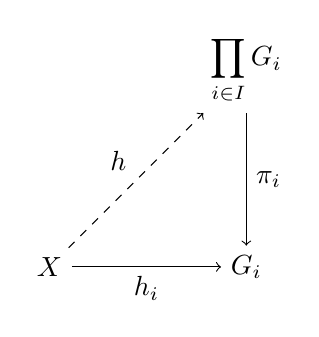
\begin{tikzpicture}[node distance=2.5cm, auto]
	\node (P) {$\displaystyle\prod_{i \in I} \bm{G_i}$};
	\node (Ci) [below of=P] {$\bm{G_i}$};
	\node (X) [left of=Ci] {$\bm{X}$};
	\draw[->] (X) to node [swap] {$h_i$} (Ci);
	\draw[->, dashed] (X) to node {$h$} (P);
	\draw[->] (P) to node {$\pi_i$} (Ci);
\end{tikzpicture}
\end{figure}
\end{proposition}
\begin{proof}
Defina a função
	\begin{align*}
	\func{h}{X}{\prod_{i \in I} G_i}{x}{(h_i(x))_{i \in I}}.
	\end{align*}
Da propriedade universal para o produto de conjuntos, $h$ é a única função tal que, para todo $i \in I$, $\pi_i \circ h = h_i$. Basta mostrar que $h$ é homomorfismo de grupos. Por simplicidade, apenas a operação $\times$ em $G$ será explicitada. Sejam $x_1,x_2 \in X$. Então, como $h_i$ são homomorfismos de grupo,
	\begin{equation*}
	h(x_1x_2) = (h_i(x_1x_2))_{i \in I} = (h_i(x_1)h_i(x_2))_{i \in I} = h(x_1)h(x_2).
	\end{equation*}
\end{proof}

\subsection{Grupo livre}

\begin{definition}
Seja $C$ um conjunto. O \emph{conjunto de inversos formais} de $C$ é o conjunto $C\inv := C \times \{-1\}$ e seus elementos são denotados $c\inv := (c,-1)$.

Uma \emph{palavra} em $C$ é uma sequência finita $(c_1,\ldots,c_n) \in C^n$. Denota-se $c_1 \cdots c_n$.
\end{definition}

Seja $p=c_1 \cdots c_n$ uma palavra em $C$. A \emph{palavra inversa} de $p$ é a palavra $p\inv := c_n\inv \cdots c_1\inv$.

\begin{definition}
Seja $C$ um conjunto e $p_1,p_2 $ palavras em $C \times \{1,-1\}$. A relação de equivalência entre as palavras $p_1$ e $p_2$ é definida por
	\begin{equation*}
	p_1 \sim p_2 \sse p_1p_2\inv \leadsto e.
	\end{equation*}	
\end{definition}

	\begin{equation*}
	C^* := \bigcup_{n \in \N} (C \times \{1,-1\})^n
	\end{equation*}
 Define-se $C^0 = \{\emptyset\}$.

	\begin{equation*}
	\ger{C} := C^*/\sim
	\end{equation*}
	
	A inclusão é definida.
	\begin{align*}
	\func{\iota}{C}{\ger{C}}{c}{[c]}.
	\end{align*}

\begin{proposition}[Propriedade Universal]
Seja $C$ um conjunto, $\bm X = (X,\star)$ um grupo e $f: C \to X$ uma função. Então existe um único homomorfismo de grupos $h: \bm{\ger{C}} \to \bm X$ tal que $h \circ \iota = f$ (o diagrama comuta).
\begin{figure}
\centering
\begin{tikzpicture}[node distance=2.5cm, auto]
	\node (C) {$C$};
	\node (G) [above of=C] {$\displaystyle\bm{\ger{C}}$};
	\node (X) [right of=C] {$\bm X$};
	\draw[->] (C) to node [swap] {$f$} (X);
	\draw[->, dashed] (G) to node {$h$} (X);
	\draw[->] (C) to node {$\iota$} (G);
\end{tikzpicture}
\end{figure}
\end{proposition}
\begin{proof}
Defina a função
	\begin{align*}
	\func{h}{\ger{C}}{X}{\left[c_1 \cdots c_n\right] }{f(c_1) \star \cdots \star f(c_n)},
	\end{align*}
de modo que $h([e])=e_X$. Então, para todo $c \in C$,
	\begin{equation*}
	h \circ \iota(c) = h (\iota(c)) = h([c])=f(c).
	\end{equation*}
Logo $h \circ \iota = f$. Para mostrar que é um homomorfismo de grupos, sejam $[c_1 \cdots c_n],$ $[d_1 \cdots d_m] \in \ger{C}$. Então
	\begin{align*}
	h([c_1 \cdots c_n][d_1 \cdots d_m]) &= h([c_1 \cdots c_nd_1 \cdots d_m]) \\
		&= f(c_1) \star \cdots \star f(c_n) \star f(d_1) \star \cdots  \star f(d_m) \\
		&= h([c_1 \cdots c_n]) \star h([d_1 \cdots d_m]).
	\end{align*}
Isso mostra a existência. Para mostrar a unicidade, seja $\overline h: \bm{\ger{C}} \to \bm X$ um homomorfismo de grupos tal que $\overline h \circ \iota = f$. Seja $[c_1 \cdots c_n] \in \ger{C}$. Como $[c_1 \cdots c_n] = [c_1] \cdots [c_n] = \iota(c_1) \cdots \iota(c_n)$, segue que
	\begin{align*}
	\overline h ([c_1 \cdots c_n]) &= \overline h(\iota(c_1) \cdots \iota(c_n)) \\
		&= \overline h(\iota(c_1)) \star \cdots \star \overline h(\iota(c_n)) \\
		&= f(c_1) \star \cdots \star f(c_n) \\
		&= h([c_1 \cdots c_n]),
	\end{align*}
o que implica que $\overline h = h$.
\end{proof}

\subsection{Coproduto de grupos}

\begin{definition}
Seja $(\bm{G_i})_{i \in I}$ uma família de grupos. O \emph{coproduto} da família $(\bm{G_i})_{i \in I}$ é o par
	\begin{equation*}
	\coprod_{i \in I} \bm{G_i} := \left(G,\times \right),
	\end{equation*}
em que $G := \ger{\coprod_{i \in I} G_i}$ é o grupo livre sobre o coproduto de conjuntos $\coprod_{i \in I} G_i$ e
	\begin{align*}
	\func{\times}{G \times G}{G}{([p_1],[p_2])}{[p_1p_2]}.
	\end{align*}
\end{definition}

\begin{proposition}[Propriedade Universal]
Sejam $(\bm{G_i})_{i \in I}$ uma família de grupos, $\bm X = (X,\star)$ um grupo e, para todo $i \in I$, $h_i: \bm{G_i} \to \bm X$ um homomorfismo de grupos. Então existe um único homomorfismo de grupos $h: \coprod_{i \in I} \bm{G_i} \to \bm X$ tal que, para todo $i \in I$, $h \circ \iota_i = h_i$ (o diagrama comuta).
\begin{figure}
\centering
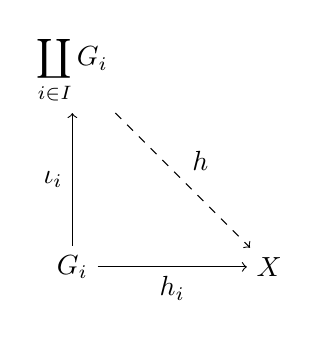
\begin{tikzpicture}[node distance=2.5cm, auto]
	\node (Ci) {$\bm{G_i}$};
	\node (S) [above of=Ci] {$\displaystyle\coprod_{i \in I} \bm{G_i}$};
	\node (X) [right of=Ci] {$\bm X$};
	\draw[->] (Ci) to node [swap] {$h_i$} (X);
	\draw[->, dashed] (S) to node {$h$} (X);
	\draw[->] (Ci) to node {$\iota_i$} (S);
\end{tikzpicture}
\end{figure}
\end{proposition}
\begin{proof}
Defina a função
	\begin{align*}
	\func{h}{\ger{\coprod_{i \in I} G_i}}{X}{\left[(g_1,i_1) \cdots (g_n,i_n)\right]}{h_{i_1}(g_1) \star \cdots \star h_{i_n}(g_n)}.
	\end{align*}

Por simplicidade, seja $G := \ger{\coprod_{i \in I} G_i}$. Para mostrar que $h$ é homomorfismo, sejam $[(g_1,i_1) \cdots (g_n,i_n)]$ e $[(g'_1,i'_1) \cdots (g'_m,i'_m)] \in G$. Então
	\begin{align*}
	&h([(g_1,i_1) \cdots (g_n,i_n)][(g'_1,i'_1) \cdots (g'_m,i'_m)]) \\
		&= h([(g_1,i_1) \cdots (g_n,i_n)(g'_1,i'_1) \cdots (g'_m,i'_m)]) \\
		&= h_{i_1}(g_1) \star \cdots \star h_{i_n}(g_n) \star h_{i'_1}(g'_1) \star \cdots \star h_{i'_n}(g'_n) \\
		&= h([(g_1,i_1) \cdots (g_n,i_n)]) \star h([(g'_1,i'_1) \cdots (g'_m,i'_m)]).
	\end{align*}
\end{proof}








































\cleardoublepage
\section{Construções específicas}

\subsection{Translações e conjugações}

\begin{definition}
Sejam $\bm G$ um grupo e $g \in G$. A \emph{conjugação} por $g$ é a função
	\begin{align*}
	\func{C_g}{G}{G}{h}{ghg\inv},
	\end{align*}
a \emph{translação à direita} por $g$ é a função
	\begin{align*}
	\func{D_g}{G}{G}{h}{hg}
	\end{align*}
e a \emph{translação à esquerda} por $g$ é a função
	\begin{align*}
	\func{E_g}{G}{G}{h}{gh}.
	\end{align*}
\end{definition}

\begin{proposition}
Sejam $\bm G$ um grupo e $g \in G$. As funções $C$, $D$ e $E$ são bijeções.
\end{proposition}
\begin{proof}
Basta mostrarmos para $D_g$ e $E_g$, pois $C_g = E_{g} \circ D_{g\inv}$. Primeiro, mostremos que as translações são homomorfismos. Para todos $g,g',h \in G$,
	\begin{equation*}
		E_{g} \circ E_{g'}(h) = gg'h = E_{gg'}(h)
	\end{equation*}
e
	\begin{equation*}
		D_{g} \circ D_{g'}(h) = hg'g = D_{g'g}(h),
	\end{equation*}
o que mostra que $E_{gg'} = E_g \circ E_{g'}$

Isso mostra que as translações à esquerda e à direita têm inversa $E_{g\inv}$ e $D_{g\inv}$, respectivamente, pois
	\begin{equation*}
		E_{g} \circ E_{g\inv} = E_{gg\inv} = \Id = E_{g\inv g} = E_{g\inv} \circ E_{g}
	\end{equation*}
e
	\begin{equation*}
		D_{g} \circ D_{g\inv} = D_{gg\inv} = \Id = D_{g\inv g} = D_{g\inv} \circ D_{g}.
	\end{equation*}
\end{proof}

\begin{proposition}
Sejam $\bm G$ um grupo e $g \in G$. A conjugação $C_g$ é isomorfismo de grupo.
\end{proposition}
\begin{proof}
Como $C_g$ é bijeção, basta mostrar que é homomorfismo de grupo. Para todos $h,h' \in G$,
	\begin{equation*}
		C_g(hh') = ghh'g\inv = ghg\inv gh'g\inv = C_g(h)C_g(h').
	\end{equation*}
\end{proof}

A \emph{conjugação} em $\bm G$ é a função
	\begin{align*}
		\func{C}{G}{\Iso{\Homo}(G)}{g}{C_g}
	\end{align*}

%A \emph{translação à direita} em $\bm G$ é a função
%	\begin{align*}
%		\func{D}{G}{\Iso{\Func}(G)}{g}{D_g}
%	\end{align*}
%
%A \emph{translação à esquerda} em $\bm G$ é a função
%	\begin{align*}
%		\func{E}{G}{\Iso{\Func}(G)}{g}{E_g}
%	\end{align*}

\subsection{Centro, automorfismos internos e externos}

\begin{definition}
Seja $\bm G$ um grupo. O \emph{centro} de $\bm G$ é o conjunto
	\begin{equation*}
		\Zen(G) := \set{g \in G}{\forall_{h \in G}\ C_g(h)=h}
	\end{equation*}
\end{definition}


Notemos que, como $C$ é homomorfismo de grupos e 
	\begin{align*}
		\Zen(G) &= \set{g \in G}{\forall_{h \in G}\ C_g(h) = h} \\
				&= \set{g \in G}{C_g = \Id} \\
				&= \nuc{C},
	\end{align*}
o centro de $\bm G$ é um subgrupo normal de $\bm G$.

\begin{definition}
Seja $\bm G$ um grupo. Um \emph{automorfismo interno} de $\bm G$ é um automorfismo da forma $C_g$ para algum $g \in G$.
\end{definition}

Pode-se mostrar que um automorfismo $\fun{h}{G}{G}$ é interno (ou seja, é conjugação por algum elemento de $G$) se, e somente se, para todo supergrupo $\bm H \geq \bm G$, esse automorfismo pode ser estendido para $\bm H$. A ida é evidente mas a volta é um pouco mais complicada\cite{art:Schupp-CharacterizationInnerAutomorphisms}.

	\begin{equation*}
	1 \to \Zen(G) \to G \to \Aut(G) \to Out(G) \to 1
	\end{equation*}


\subsection{Centralizador e normalizador}






\subsection{Produto semidireto}

\begin{definition}
Sejam $\bm G$ e $\bm H$ grupos e $A\colon \bm G \age \bm H$ uma ação do grupo $\bm G$ sobre o grupo $\bm H$. O \emph{produto semidireto} (à esquerda) de $\bm H$ por $\bm G$ com respeito a $A$ é o grupo
	\begin{equation*}
		\bm G \ltimes_A \bm H := (G \times H,\times_{G \ltimes_A H},\div_{G \ltimes_A H},\id_{G \ltimes_A H})
	\end{equation*}
em que
	\begin{align*}
		\func{\times_{G \ltimes_A H}}{(G \times H) \times (G \times H)}{G \times H}{((g,h),(g',h'))}{(gg',hA_g(h'))},
	\end{align*}
	\begin{align*}
		\func{\div_{G \ltimes_A H}}{G \times H}{G \times H}{(g,h)}{(g\inv,A_{g\inv}(h\inv))}
	\end{align*}
e
	\begin{equation*}
		\id_{G \ltimes_A H} := (\id_G,\id_H).
	\end{equation*}
Por simplicidade, denotamos $G \ltimes H$ quando a ação está subentendida no contexto.

%O \emph{produto semidireto} (à direita) de $\bm H$ por $\bm G$ com respeito a $A$ é o grupo
%		\begin{equation*}
%			\bm H \rtimes_A \bm G := (H \times G,\times_A,\div_A,\id_A)
%		\end{equation*}
%	em que
%		\begin{align*}
%			\func{\times_A}{(H \times G) \times (H \times G)}{H \times G}{((h,g),(h',g'))}{(A_g(h'),g'g)}
%		\end{align*}
\end{definition}

O produto semidireto à direita é definido analogamente e denotado $\bm H \rtimes_A \bm G$, com
	\begin{align*}
		\func{\times_{H \rtimes G}}{(H \times G) \times (H \times G)}{H \times G}{((h,g),(h',g'))}{(A_g(h')h,gg')}
	\end{align*}
e as mesmas inversa e identidade do caso à esquerda. Vale ressaltar que com uma ação do grupo $\bm G$ sobre o grupo $\bm H$ queremos dizer um homomorfismo de grupos
	\begin{equation*}
		A\colon \bm G \to \Iso{\Homo}(\bm H),
	\end{equation*}
em que $\Iso{\Homo}(\bm H)$ é o grupo dos automorfismos de grupo de $\bm H$.

% Qual a relação da ação ser à esquerda/direita com o produto semidireto ser à esquerda/direita?

\begin{exercise}
Sejam $\bm G$ e $\bm H$ grupos e $A\colon \bm G \age \bm H$ uma ação do grupo $\bm G$ sobre o grupo $\bm H$.
	\begin{enumerate}
		\item O produto semidireto $\bm G \ltimes_A \bm H$ é um grupo.
		
		\item $\bm G \simeq \bm G \ltimes \bm{\{\id_H\}} \leq \bm G \ltimes \bm H$, e $\bm G \ltimes \bm{\{\id_H\}} \ide \bm G \ltimes \bm H$ se, e somente se, $\bm G \ltimes \bm H = \bm G \times \bm H$ (ou $A=\Id_H$);
		
		\item $\bm H \simeq \bm{\{\id_G\}} \ltimes \bm H \ide \bm G \ltimes \bm H$;
	\end{enumerate}
\end{exercise}

\begin{example}
	\begin{enumerate}
		\item O produto direto de grupos $\bm G$ e $\bm H$ é um produto semidireto cuja ação é a função constante
	\begin{align*}
		\func{\Id_H}{G}{\Iso{\Homo}(H)}{g}{
			\begin{aligned}[t]
				\func{\Id_H}{H}{H}{h}{h}
			\end{aligned}
		}
	\end{align*}

	\item Seja $n \in \N$. $\OO(n) \simeq \S^0 \ltimes \SO(n)$ com ação dada por
		\begin{align*}
			\func{A}{\S^0}{\Aut(\SO(n))}{i}{
				\begin{aligned}[t]
					\func{C_{\Id_{n-1} \oplus i}}{\SO(n)}{\SO(n)}{N}{(\Id_{n-1} \oplus i) \circ N \circ (\Id_{n-1} \oplus i)\inv}.
				\end{aligned}
			}
		\end{align*}
	A transformação linear $\Id_{n-1} \oplus i \in \OO(n)$ é uma reflexão de $\R^n$ que pode ser representada pela matrix
		\begin{equation*}
			\begin{pmatrix}
				\Id_{n-1}	&	0 \\
				0			&	i
			\end{pmatrix}.
		\end{equation*}
	\end{enumerate}
\end{example}













\subsection{Grupo simples e subgrupo normal maximal}

\begin{definition}
Um \emph{grupo simples} é um grupo não-trivial $\bm G$ cujos únicos subgrupos normais são $\bm{\{1\}}$ e $\bm G$.
\end{definition}

\begin{definition}
Seja $\bm G$ um grupo. Um subgrupo normal \emph{maximal} de $\bm G$ é um subgrupo normal próprio $\bm M \idepro \bm G$ que satisfaz
	\begin{enumerate}
	\item (Maximalidade) Para todo $\bm N \ide \bm G$,
		\begin{equation*}
		M \subseteq N \Rightarrow N = M \text{\ \ ou\ \ } N = G.
		\end{equation*}
	\end{enumerate}
\end{definition}

\begin{proposition}
Sejam $\bm G$ um grupo e $\bm M \ide \bm G$ um subgrupo normal. Então $\bm M$ é maximal se, e somente se, $\bm{G/M}$ é simples.
\end{proposition}
\begin{proof} Consideremos a projeção canônica
	\begin{align*}
	\func{\pi}{G}{\quo{G}{M}}{g}{gM}.
	\end{align*}
	\begin{enumerate}
		\item [($\Rightarrow$)] Suponhamos que $\bm M$ é maximal. Então $\bm M$ é um subgrupo próprio, o implica que $\bm{G/M}$ é não-trivial. Seja $\bm N \ide \bm{G/M}$. Sabemos que $\bm{\pi^{-1}(N)} \ide \bm G$ (\ref{alge:prop.gru.hominv}). Como $[e] \in N$, então $\pi^{-1}(1) \subseteq \pi^{-1}(N)$. Notando que $\pi^{-1}([1])=\nuc(\pi) = M$, segue que $M \subseteq \pi^{-1}(N)$. Como $\bm M$ é maximal, segue que $\pi^{-1}(N) = N$ ou $\pi^{-1}(N) = G$. Notemos que $N=\pi(\pi^{-1}(N))$, pois $\pi$ é sobrejetiva. No primeiro caso, $N = \pi(\pi^{-1}(N)) = \pi(M) = \{[1]\}$. No segundo caso, $N = \pi(\pi^{-1}(N)) = \pi(G) = G/M$. Portanto $\bm{G/M}$ é simples.
		
		\item [($\Leftarrow$)] Suponhamos que $\bm{G/M}$ é simples. Seja $\bm N \ide \bm G$ tal que $M \subseteq N$. Como $\pi$ é homomorfismo de grupos sobrejetivo, segue que $\pi(N) \ide \bm{G/M}$ (\ref{alge:prop.gru.hom}). Como $\bm{G/M}$ é simples, então $\pi(N) = \{[e]\}$ ou $\pi(N) = G/M$. No primeiro caso, $N = \nuc(\pi) = M$. No segundo caso, $N = \pi^{-1}(\pi(N)) = \pi^{-1}(N) = G$. Logo $\bm M$ é maximal.
	\end{enumerate}
\end{proof}

\begin{conjecture}
Sejam $\bm G$ um grupo e $\bm N \idepro \bm G$ um subgrupo normal próprio. Então $\bm G$ tem subgrupo normal maximal.
\end{conjecture}
\begin{proof}
Usaremos o lema de Zorn. Seja $P \subseteq \p(G)$ o conjunto de todos os subconjuntos $S \subset G$ tais que $\bm S \idepro \bm G$. Então $(P,\subseteq)$ é um conjunto parcialmente ordenado com a contenção de conjuntos usual. Agora, seja $(C)_{i \in I}$ uma cadeia de $(P,\subseteq)$. Consideremos o conjunto $C := \bigcup_{i \in I} C_i$. Como 

Notemos que $P$ não é vazio, pois $N \in P$. Seja



Então $P$ tem elemento maximal.
\end{proof}






\subsection{Sequência subnormal}

\begin{definition}
Seja $\bm G$ um grupo. Uma \emph{sequência subnormal} de $\bm G$ é uma sequência finita $(\bm{N_i})_{i \in [n]}$ de subgrupos de $\bm G$ que satisfaz
	\begin{equation*}
	\bm{\{1\}} = \bm{N_0} \ide \cdots \ide \bm{N_{n-1}} = \bm G.
	\end{equation*}
O grupo $\bm{N_{i+1}/N_i}$ é o $i$-ésimo \emph{grupo fator} da sequência.
Uma \emph{sequência normal} é uma sequência subnormal em que, para todo $i \in [n]$, $\bm{N_i} \ide \bm G$.

Uma sequência subnormal \emph{estrita} de $\bm G$ é uma sequência subnormal $(\bm{N_i})_{i \in [n]}$ de $\bm G$ que satisfaz
	\begin{equation*}
	\bm{\{1\}} = \bm{N_0} \idepro \cdots \idepro \bm{N_{n-1}} = \bm G.
	\end{equation*}
	
O \emph{comprimento} de uma sequência subnormal estrita é o número $n$.
\end{definition}



\subsection{Conjunto gerador}

\begin{definition}
Seja $\bm G$ um grupo e $S \subseteq G$ um conjunto. O grupo \emph{gerado} por $S$ é o grupo $\bm{\langle S \rangle} \leq \bm G$ em que
	\begin{equation*}
	\langle S \rangle := \set{s_1 \cdots s_n}{n \in \N,\ s_i \in S \text{\ \ ou\ \ } s_i\inv \in S}.
	\end{equation*}
	\begin{equation*}
	\langle S \rangle := \set{\bigopb_{i \in [n]} s_i}{n \in \N,\ s_i \in S \text{\ \ ou\ \ } s_i\inv \in S}.
	\end{equation*}
\noindent
Um \emph{conjunto gerador} de $\bm G$ é um conjunto $S \subseteq G$ tal que $\langle S \rangle = G$.
\end{definition}









\section{Ação de grupos}

\subsection{Grupo simétrico}

Para falar de ação de grupo, primeiro demonstraremos que o conjunto de bijeções de um conjunto para si mesmo é um grupo com as operações de composição, inversa de função e função identidade.

\begin{definition}
Seja $C$ um conjunto. O \emph{grupo simétrico} (ou \emph{grupo de bijeções}) de $C$ é a lista
	\begin{equation*}
	\Iso{\bm{\Func}}(C) = (\Iso{\Func}(C),\circ,\inv,\Id),
	\end{equation*}
em que $\Iso{\Func}(C)$ é o conjunto de bijeções de $C$ para $C$, $\circ$ é a composição de funções, $\inv$ é a inversa de funções e $\Id$ é a função identidade.
%Seja $\alpha$ um número cardinal. Para $C = \alpha$, usa-se a notação $\sime_{\alpha} := \Iso{\Func}(\alpha)$.
\end{definition}

\begin{proposition}
Seja $C$ um conjunto. O grupo simétrico $\Iso{\bm{\Func}}(C)$ é um grupo.
\end{proposition}
\begin{proof}
Se $C=\emptyset$, então $\Iso{\Func}(C)=\{\emptyset\}$. Assim, como $\emptyset \circ \emptyset = \emptyset$, segue que $\circ$ é operação binária em $\{\emptyset\}$. Ainda, segue que $\circ$ é associativa, pois $(\emptyset \circ \emptyset) \circ \emptyset = \emptyset \circ (\emptyset \circ \emptyset)$; tem elemento neutro $\emptyset$, pois $\emptyset \circ \emptyset = \emptyset$, e que todo elemento tem inverso, pois $\emptyset\inv = \emptyset$.

Suponhamos, então, que $C \neq \emptyset$ e sejam $p_1,p_2 \in \Iso{\Func}(C)$. Como $p_1$ e $p_2$ são bijeções, a função $p_2 \circ p_1: C \to C$ é uma bijeção entre $C$ e $C$ (\ref{prop:comp.func.inj} e \ref{prop:comp.func.sobr}) e, portanto, $p_2 \circ p_1 \in \Iso{\Func}(C)$. Isso mostra que $\circ$ é uma operação binária em $\Iso{\Func}(C)$.
	\begin{enumerate}
		\item A composição de funções é associativa, pois, para todos $p_1,p_2,p_3 \in \Iso{\Func}(C)$, $p_3 \circ (p_2 \circ p_1) = (p_3 \circ p_2) \circ p_1$ (\ref{prop:comp.func.asso}).

		\item Ainda, notemos que $\Id_C$ é o elemento neutro de $\Iso{\bm{\Func}}(C)$, pois, para todo $p \in \Iso{\Func}(C)$, vale $p \circ \Id_C = \Id_C \circ p = p$ (\ref{prop:id.comp.func}).

		\item Por fim, como $p$ é uma bijeção, existe função inversa $p\inv: C \to C$ que é bijeção entre $C$ e $C$ (\ref{prop:func.inv.esq} e \ref{prop:func.inv.dir}); logo existe $p\inv \in \Iso{\Func}(C)$ tal que $p \circ p\inv = p\inv \circ p = \Id_C$.
	\end{enumerate}
Portanto concluímos que $\Iso{\bm{\Func}}(C)$ é um grupo.
\end{proof}

\begin{proposition}
	Sejam $A$ e $B$ conjuntos tais que $\card{A} = \card{B}$. Então
	\begin{equation*}
	\Iso{\bm{\Func}}(A) \simeq \Iso{\bm{\Func}}(B).
	\end{equation*}
\end{proposition}
\begin{proof}
	Seja $\phi: A \to B$ uma bijeção e considere a função
	\begin{align*}
	\func{h}{\Iso{\Func}(A)}{\Iso{\Func}(B)}{p}{\phi \circ p \circ \phi\inv}.
	\end{align*}
Primeiro notemos que $h$ é homomorfismo de grupos. Sejam $p_1,p_2 \in \Iso{\Func}(A)$. Então
	\begin{align*}
	h(p_2 \circ p_1)(c) &= \phi \circ (p_2 \circ p_1) \circ \phi^{-1} \\
			&= \phi \circ (p_2 \circ \phi\inv \circ \phi \circ p_1) \circ \phi^{-1} \\
			&= (\phi \circ p_2 \circ \phi\inv) \circ (\phi \circ p_1 \circ \phi\inv) \\
			&= h(p_2) \circ h(p_1).
	\end{align*}
Portanto $h$ é um homomorfismo de grupos entre $\Iso{\bm{\Func}}(A)$ e $\Iso{\bm{\Func}}(B)$.

Agora notemos que $h$ é uma bijeção. A inversa de $h$ é a função
	\begin{align*}
	\func{h\inv}{\Iso{\Func}(B)}{\Iso{\Func}(A)}{p}{\phi\inv \circ p \circ \phi},
	\end{align*}
pois, para todo $p \in \Iso{\Func}(B)$,
	\begin{align*}
	(h \circ h\inv) (p) &= h (h\inv(p)) \\
			&= \phi \circ h\inv(p) \circ \phi\inv \\
			&= \phi \circ (\phi\inv \circ p \circ \phi) \circ \phi\inv \\
			&= p \\
			&= 1_{\Iso{\Func}(B)}(p),
	\end{align*}
o que mostra que $h \circ h\inv = 1_{\Iso{\Func}(B)}$, e, para todo $p \in \Iso{\Func}(A)$,
	\begin{align*}
	(h\inv \circ h) (p) &= h\inv (h(p)) \\
			&= \phi\inv \circ h(p) \circ \phi \\
			&= \phi\inv \circ (\phi \circ p \circ \phi\inv) \circ \phi \\
			&= p \\
			&= 1_{\Iso{\Func}(A)}(p),
	\end{align*}
o que mostra que $h\inv \circ h = 1_{\Iso{\Func}(A)}$. Assim, está provado que $h$ é isomorfismo entre $\Iso{\bm{\Func}}(A)$ e $\Iso{\bm{\Func}}(B)$.
\end{proof}

	Essa proposição mostra que podemos estudar somente os grupos simétricos dos números cardinais, pois isso será equivalente a estudar qualquer grupo simétrico. Em particular, para todo conjunto finito, podemos estudar seu grupo simétrico considerando somente o grupo simétrico $\bm\sime_n$, em que $n$ é o número de elementos do conjunto. A partir de agora, as proposições serão considerando esses grupos $\bm\sime_n$.

\begin{theorem}
	Seja $\bm G$ um grupo. Então
	\begin{equation*}
	\bm G \lesssim \Iso{\bm{\Func}}(G).
	\end{equation*}
\end{theorem}
\begin{proof}
	Consideremos a função
	\begin{align*}
	\func{h}{G}{\Iso{\Func}(G)}{g}{
		\begin{aligned}[t]
		\func{h(g)}{G}{G}{x}{g \times x}
		\end{aligned}
	}
	\end{align*}
Primeiro, devemos mostrar que $h(g) \in \Iso{\Func}(G)$, para que $h$ esteja bem definida. Para isso, notemos que $h(g)$ está bem definida, já que, para todo $x \in G$, $g \times x \in G$. Ainda, $h(g)$ é uma bijeção, pois $h(g)\inv = h(g\inv)$, já que, para todo $x \in G$,
	\begin{equation*}
	(h(g) \circ h(g)\inv)(x) = h(g)((h(g)\inv)(x)) = h(g)(g\inv \times x) = g \times g\inv \times x = x = 1_G,
	\end{equation*}
o que mostra que $h(g) \circ h(g)\inv = 1_G$, e
	\begin{equation*}
	(h(g)\inv \circ h(g))(x) = h(g)\inv((h(g)(x)) = h(g)\inv(g \times x) = g\inv \times g \times x = x = 1_G,
	\end{equation*}
o que mostra que $h(g)\inv \circ h(g) = 1_G$. Isso mostra que $h(g)$ é uma bijeção e, portanto, $h(g) \in \Iso{\Func}(G)$.

	Agora, notemos que $h$ é um homomorfismo de grupos, pois, para todos $g_1,g_2 \in G$, segue que, para todo $x \in G$,
	\begin{align*}
	h(g_1 \times g_2)(x) &= (g_1 \times g_2) \times x \\
	&= g_1 \times (g_2 \times x) \\
	&= h(g_1)(g_2 \times x) \\
	&= h(g_1)(h(g_2)(x)) \\
	&= (h(g_1) \circ h(g_2))(x),
	\end{align*}
o que mostra que $h(g_1 \times g_2) = h(g_1) \circ h(g_2)$. Por fim, notemos que $h$ é injetiva, já que, se $g \in G$ é tal que $h(g)=id_G$, então, para todo $x \in G$,
	\begin{equation*}
	g \times x = h(g)(x) = 1_G(x) = x,
	\end{equation*}
o que mostra que $g=e_G$ e, portanto, que $\nuc(h)=\{e_G\}$.
\end{proof}

	Esse teorema é um teorema muito importante, pois ele mostra que, de certa forma, todo grupo é um subconjunto de permutações. Por causa disso que grupos são pensados como os objetos algébricos que modelam a simetria.

\subsection{Ações}

A noção de uma ação de grupo, de certa forma, generaliza uma estratégia usada na demonstração do teorema de que todo grupo é isomorfo a um subgrupo de seu grupo simétrico.

\begin{definition}
Sejam $\bm G$ um grupo e $X$ um conjunto. Uma \emph{ação} de $\bm G$ em $X$ é um homomorfismo de grupos
	\begin{align*}
	\func{A}{G}{\Iso{\Func}(X)}{g}{
		\begin{aligned}[t]
		\func{g\pt}{X}{X}{x}{g\pt x}.
		\end{aligned}
	}
	\end{align*}
Denota-se $\acao{A}{\bm G}{X}$. Diz-se que o grupo $\bm G$ \emph{age} no conjunto $X$, e denota-se $\bm G \age X$, se, e somente se, existe ação de $\bm G$ em $X$.
%O grupo $\bm G$ é o \emph{grupo de funções} e o conjunto $X$ é um \emph{$\bm G$-conjunto}.
\end{definition}

A definição acima é uma definição muito simplificada pois ela depende de conceitos um pouco mais complexos, como de homomorfismo de grupos e de grupo de bijeções. A proposição abaixo mostra como essa definição é equivalente a uma definição mais explícita de ação de grupo que também é comumente usada.

\begin{proposition}
Sejam $X$ um conjunto e $\bm G$ um grupo. Então $\bm G \age X$ se, e somente se, existe uma função
	\begin{align*}
	\func{\pt}{G \times X}{X}{(g,x)}{g\pt x}
	\end{align*}
que satisfaz
\begin{enumerate}
\item (Identidade) Para todo $x \in X$,
	\begin{equation*}
	e \pt x = x;
	\end{equation*}
\item (Compatibilidade) Para todos $g_0,g_1 \in G$ e $x \in X$,
	\begin{equation*}
	(g_1g_0) \pt x = g_1 \pt (g_0 \pt x).
	\end{equation*}
\end{enumerate}
\end{proposition}
\begin{proof}
Se existe ação $\acao{A}{\bm G}{X}$, basta definir $g \pt x := A(g)(x)$ e segue que $e\pt = 1$ e $(g_1g_0) \pt = (g_1 \pt) \circ (g_0 \pt)$. Reciprocamente, definimos a ação $A$ a partir de $\pt$ da mesma forma e, se $g_0,g_1 \in G$ e $x \in X$, segue que
	\begin{equation*}
	A(g_1g_0)(x) =(g_1g_0) \pt x = g_1 \pt (g_0 \pt x) = A(g_1)(A(g_0)(x)) = A(g_1) \circ A(g_0)(x),
	\end{equation*}
logo $A(g_1g_0)=A(g_1) \circ A(g_0)$.
\end{proof}

Essa proposição é geralmente considerada a definição de uma ação \emph{à esquerda} de $\bm G$ em $X$ por causa da posição em que a composição ocorre. Analogamente, uma ação à direita pode ser definida, mas toda ação à direita pode ser traduzida em uma ação à esquerda, de modo que é suficiente estudar somente ações à esquerda. É comum, ainda, estudar ações em conjuntos $X$ com alguma estrutura adicional, geralmente uma topologia. Nesse caso, exige-se que a ação seja uma função contínua, mas também é necessário que $G$ tenha uma estrutura topológica, portanto isso não será definido com cuidado agora.

\subsection{Órbitas e estabilizadores}

\begin{definition}
Sejam $X$ um conjunto, $\bm G$ um grupo, $\bm G \age X$ e $x \in X$. A \emph{órbita} de $x$ sob $\bm G$ é o conjunto
	\begin{equation*}
	G \pt x := \set{g\pt x}{g \in G}.
	\end{equation*}
\end{definition}

\begin{definition}
Sejam $X$ um conjunto, $\bm G$ um grupo, $A: \bm G \age X$ e $x \in X$. O \emph{estabilizador} de $x$ é
	\begin{equation*}
	G_x = \set{g \in G}{g\pt x = x} = A\inv(\{1\}) = \nuc(A).
	\end{equation*}
\end{definition}

O estabilizador de $x$ é um grupo e por isso é chamado de \emph{subgrupo estabilizador} de $\bm G$ com respeito a $x$, e também é conhecido como \emph{grupo de isotropia} de $x$.







\subsection{Permutações finitas}


\begin{exercise}
Seja $n \in \N$. Então $|\sime_n|=n!$.
\end{exercise}


\begin{definition}
Seja $n \in \N$. Uma \emph{permutação} de $n$ objetos é um elemento $p \in \sime_n$, denotado por
	\begin{equation*}
	p = \begin{pmatrix}
				1 & 2 & \cdots & n-1 & n \\
				p(1) & p(2) & \cdots &  p(n-1)  & p(n)
			\end{pmatrix}.
	\end{equation*}
\end{definition}

\begin{notation}
Seja $n \in \N$. A composição de duas permutações $p_1,p_2 \in \sime_n$, quando representadas na notação acima, é denotada
	\begin{equation*}
	p_2 \circ p_1 = \bigl(\begin{smallmatrix}
				1 & 2 & \cdots & n-1 & n \\
				p_2(1) & p_2(2) & \cdots &  p_2(n-1)  & p_2(n)
			\end{smallmatrix}\bigr)
			\bigl(\begin{smallmatrix}
				1 & 2 & \cdots & n-1 & n \\
				p_1(1) & p_1(2) & \cdots &  p_1(n-1)  & p_1(n)
			\end{smallmatrix}\bigr).
	\end{equation*}
\end{notation}

\begin{definition}
	Sejam $n \in \N$ e $p \in \sime_n$. A \emph{matriz de permutação} de $p$ é a matriz $[p] \in \M_n (\Z)$ cujas entradas são dadas por
	\begin{equation*}
		[p]_{i,j} = \delta_{i,p(j)} = \begin{cases}
												1 & i=p(j) \\
												0 & i \neq p(j).
												\end{cases}
	\end{equation*}
	O \emph{conjunto das matrizes de permutação} de $\sime_n$ é o conjunto
	\begin{equation*}
		[\sime_n] := \set{[p]}{p \in \sime_n}.
	\end{equation*}
\end{definition}

\begin{proposition}
	Seja $n \in \N$. Então o par $\bm{[\sime_n]}=([\sime_n],\cdot)$, em que $\cdot$ é o produto de matrizes, é um grupo, e
	\begin{equation*}
	\bm{\sime_n} \simeq \bm{[\sime_n]}.
	\end{equation*}
\end{proposition}
\begin{proof}
	Primeiro, notemos que, para todos $p,q \in \sime_n$,
	\begin{equation*}
	[p][q]_{i,j} = \sum_{k=0}^{n-1} [p]_{i,k}[q]_{k,j} = \sum_{k=0}^{n-1} \delta_{i,p(k)}\delta_{k,p(j)}.
	\end{equation*}
	Mas o produto $\delta_{i,p(k)}\delta_{k,p(j)}$ é igual a 1 se, e somente se, $i=p(k)$ e $k=q(j)$. Como $p$ é bijeção, a segunda condição é equivalente a $p(k)=pq(j)$, e isso mostra que as duas condições são equivalentes a $i=p(k)=pq(j)$. Como $p$ é bijeção, para cada $i \in [n]$, $k=p\inv(i)$ é o único $k \in [n]$ tal que a condição é satisfeita, e segue que
	\begin{equation*}
	[p][q]_{i,j} = \sum_{k=1}^n \delta_{i,p(k)}\delta_{k,p(j)} = \sum_{k=1}^n \delta_{i,pq(j)} = [pq]_{i,j}.
	\end{equation*}
e, como $pq \in \sime_n$, então $[p][q]=[pq] \in [\sime_n]$. Isso mostra que o produto de matrizes é uma operação binária em $[\sime_n]$. Agora, disso segue que $[p][p\inv]=[pp\inv]=[id]$

%MOSTRAR QUE O INVERSO DE P ESTA NO GRUPO




Disso, segue que $\bm{[\sime_n]}$ é um grupo, pois é subgrupo de $\M_n(\Z)$. Por fim, consideremos a função
	\begin{align*}
	\func{h}{\sime_n}{[\sime_n]}{p}{[p]}.
	\end{align*}
Note que que $h$ é homomorfismo, pois, para todos $p,q \in \sime_n$,
	\begin{equation*}
	h(pq) = [pq]= [p][q] = h(p)h(q).
	\end{equation*}
Ainda, $h$
\end{proof}

\begin{definition}
	Sejam $n \in \N$, $p \in \sime_n$ e $m \in [n]$. A \emph{órbita de $m$ sob $p$} é o conjunto
	\begin{equation*}
	\orb_p(m) := \set{p^k(m)}{k \in \Z}.
	\end{equation*}
O \emph{período} da órbita $\orb_p(m)$ é o número $\card{\orb_p(m)}$. Uma \emph{órbita trivial} é uma órbita de período $1$. Uma órbita de $p$ é a órbita de um elemento $m \in [n]$ sob $p$.

	O \emph{conjunto de órbitas} de $p$ é o conjunto
	\begin{equation*}
	\orb_p := \set{\orb_p(m)}{m \in [n]}.
	\end{equation*}
\end{definition}

\begin{proposition}
	Sejam $n \in \N$ e $p \in \sime_n$. O conjunto $\orb_p$ é uma partição de $[n]$.
\end{proposition}
\begin{proof}
	Primeiro, notemos que $m \in \orb_p(m)$ e, portanto, $\emptyset \nsubseteq \orb_p$. Ainda, $\bigcup_{m \in [n]} \orb_p(m) = [n]$, já que, para todo $m \in [n]$, $m \in \orb_p(m)$, o que mostra que $[n] \subseteq \bigcup_{m \in [n]}$ e, para todo $l \in \bigcup_{m \in [n]} \orb_p(m)$, existe $m \in [n]$ tal que $l \in \orb_p(m)$ e, portanto, existe $k \in \N$ tal que $l=p^k(m) \in [n]$, o que mostra que $\bigcup_{m \in [n]} \subseteq [n]$. Por fim, sejam $o_1,o_2 \in \orb_p$. Então existem $m_1,m_2 \in [n]$ tais que $o_1=\orb_p(m_1)$ e $o_2=\orb_p(m_2)$. Se existe $l \in \orb_p(m_1) \cap \orb_p(m_2)$, então existem $k_1,k_2 \in \Z$ tais que $l=p^{k_1}(m_1)=p^{k_2}(m_2)$. Assim, segue que $m_1=p^{k_2-k_1}(m_2)$ e, portanto, $m_1 \in \orb_p(m_2)$. Mas isso implica que $\orb_p(m_1) \subseteq \orb_p(m_2)$; a inclusão contrária é análoga e concluímos que $\orb_p(m_1) = \orb_p(m_2)$. Logo $\orb_p$ é uma partição de $[n]$.
\end{proof}

\subsubsection{Ciclos e transposições}

\begin{definition}
	Sejam $n,k \in \N$. Um \emph{ciclo} de $\sime_n$ é um elemento $c \in \sime_n$ para o qual existe $m \in [n]$ tal que, para todo $m' \in [n]$, $c(m')=m'$ ou existe $d \in [n]$ tal que $m'=c^d(m)$. O \emph{comprimento} de um ciclo é a ordem desse ciclo. Um ciclo $c$ cujo comprimento é $k$ é denotado
	\begin{equation*}
	c = \bigl(m \ c(m) \ c^2(m) \ \cdots \  c^{k-2}(m) \ c^{k-1}(m)\bigr).
	\end{equation*}
\end{definition}


\begin{proposition}
	Sejam $n \in \N$.
	\begin{enumerate}
	\item Se $c_1,c_2 \in \sime_n$ são ciclos disjuntos, então $c_2 \circ c_1 = c_1 \circ c_2$.
	\end{enumerate}
\end{proposition}

\begin{proposition}[Fatoração de Permutação]
	Seja $n \in \N$ e $p \in \sime_n$. Então existem únicos ciclos $c_1,\ldots,c_k \in \sime_n$ disjuntos dois a dois tais que $p=c_1 \circ \cdots \circ c_k$.
\end{proposition}
\begin{proof}
	Seja $k := \card{\orb_p}$. O conjunto $\orb_p$ particiona $[n]$. Sejam $(o_k)_{i \in [k]}$ uma indexação de $\orb_p$ e $m_1,\cdot,m_k \in [n]$ tais que $o_i=\orb_p(m_i)$ para todo $i \in [k]$, e seja $k_i := \card{\orb_p(m_i)}$. Definamos $c_i :=  \bigl( m_i \ \cdots \  p^{k_i-1}(m_i)\bigr)$. Então segue que
	\begin{equation*}
	p = \bigtimes_{i=1}^k \bigl( m_i \ \cdots \  p^{k_i-1}(m_i)\bigr) = \bigtimes_{i=1}^k c_i.
	\end{equation*}
\end{proof}

%\subsection{Grupo alternado}



%\subsection{Grupos cíclicos}

%\subsection{Grupos diedrais}







\section{Grupo linear geral}

\begin{definition}
Sejam $\bm C$ um corpo e $n \in \N$. O \emph{grupo linear geral} de $\bm C$ de ordem $n$ é o conjunto
	\begin{equation*}
	\GL_n(\bm C) := \set{M \in \M_{n\times n}(\bm C)}{\det M \neq 0}.
	\end{equation*}
Se $\bm V$ é um espaço vetorial finito de dimensão $d$ sobre um corpo $\bm C$, o \emph{grupo linear geral} de $\bm V$ é
	\begin{equation*}
	\GL(\bm V) := \GL_n(\bm C).
	\end{equation*}
\end{definition}

Como $\det(AB) = \det(A)\det(B)$ e as matrizes invertíveis são as que têm determinante não nulo, segue que o conjunto acima forma um grupo com respeito ao produto de matrizes.

\begin{definition}
Sejam $\bm C$ um corpo e $n \in \N$. O \emph{grupo linear especial} de $\bm C$ de ordem $n$ é o conjunto
	\begin{equation*}
	\SL_n(\bm C) := \set{M \in \GL(n,\bm C)}{\det M =1}.
	\end{equation*}
\end{definition}


\section{Representação de grupos}

\begin{definition}
Sejam $\bm G$ um grupo e $\bm V$ um espaço vetorial sobre um corpo $\bm C$. Uma \emph{representação} de $\bm G$ em $\bm V$ é um homomorfismo de grupos
	\begin{equation*}
	\rho: \bm G \to \GL(\bm V).
	\end{equation*}
O espaço $\bm V$ é o \emph{espaço de representação} e a dimensão de $\bm V$ é a \emph{dimensão da representação}.
\end{definition}

\begin{definition}
Seja $\bm V$ um espaço vetorial sobre um corpo $\bm C$.
\end{definition}

\section{Sequências Exatas}

\begin{definition}
Uma \emph{sequência crescente finita} de homomorfismos de grupo é uma sequência de homomorfismos de grupo $(h_i)_{i \in [n]}$ tal que $n \in \N$ e, para todo $i \in [n]$, $\bm G_i$ e $\bm G_{i+1}$ são grupos e $\fun{h_i}{\bm G_i}{\bm G_{i+1}}$. Denota-se
	\begin{equation*}
	G_0 \overset{h_0}{\longrightarrow} \cdots \overset{h_{i-1}}{\longrightarrow} G_i \overset{h_i}{\longrightarrow} G_{i+1} \overset{h_{i+1}}{\longrightarrow} \cdots \overset{h_{n-1}}{\longrightarrow} G_{n}.
	\end{equation*}
Uma \emph{sequência decrescente finita} de homomorfismos de grupo é uma sequência de homomorfismos de grupo $(h_i)_{i \in [n]}$ tal que $n \in \N$ e, para todo $i \in [n]$, $\bm G_i$ e $\bm G_{i+1}$ são grupos e $\fun{h_i}{\bm G_{i+1}}{\bm G_i}$. Denota-se
	\begin{equation*}
	G_n \overset{h_{n-1}}{\longrightarrow} \cdots \overset{h_{i+1}}{\longrightarrow} G_{i+1} \overset{h_i}{\longrightarrow} G_i \overset{h_{i-1}}{\longrightarrow} \cdots \overset{h_0}{\longrightarrow} G_0.
	\end{equation*}

Uma \emph{sequência crescente infinita} de homomorfismos de grupo é uma sequência de homomorfismos de grupo $(h_i)_{i \in \N}$ tal que, para todo $i \in \N$, $\bm G_i$ é grupo e $\fun{h_i}{\bm G_i}{\bm G_{i+1}}$. Denota-se
	\begin{equation*}
	G_0 \overset{h_0}{\longrightarrow} \cdots \overset{h_{i-1}}{\longrightarrow} G_i \overset{h_i}{\longrightarrow} G_{i+1} \overset{h_{i+1}}{\longrightarrow} \cdots .
	\end{equation*}
Uma \emph{sequência decrescente infinita} de homomorfismos de grupo é uma sequência de homomorfismos de grupo $(h_i)_{i \in \N}$ tal que, para todo $i \in \N$, $\bm G_i$ é grupo e $\fun{h_i}{\bm G_{i+1}}{\bm G_i}$. Denota-se
	\begin{equation*}
	\cdots \overset{h_{i+1}}{\longrightarrow} G_{i+1} \overset{h_i}{\longrightarrow} G_i \overset{h_{i-1}}{\longrightarrow} \cdots \overset{h_0}{\longrightarrow} G_0.
	\end{equation*}
\end{definition}

Vamos usar em geral a notação crescente finita, mas sempre ficará claro como adaptar a demonstração para os outros casos.

\begin{definition}
Uma \emph{sequência exata} de homomorfismos de grupo é uma sequência de homomorfismo de grupos $(h_i)_{i \in [n]}$ tal que, para todo $i \in [n]$,
	\begin{equation*}
	\im(h_i) = \nuc(h_{i+1}).
	\end{equation*}
\end{definition}

\begin{exercise}
	\begin{enumerate}
	\item A sequência $\funseq{\{1\}}{1} \funseq{G}{h} G'$ é exata se, e somente se, $h$ é monomorfismo;
	\item A sequência $\funseq{G'}{h} \funseq{G}{1} \{1\}$ é exata se, e somente se, $h$ é epimorfismo;
	\item A sequência $\funseq{\{1\}}{1} \funseq{G}{h} \funseq{G'}{1} \{1\}$ é exata se, e somente se, $h$ é isomorfismo;
	\item A sequência $\funseq{\{1\}}{1} \funseq{G}{h} \funseq{G'}{h'} \funseq{G''}{1} \{1\}$ é exata se, e somente se,
		\begin{equation*}
		G'' \simeq \quo{G'}{h(G)}.
		\end{equation*}
	\end{enumerate}
\end{exercise}

\begin{definition}
Uma \emph{sequência exata curta} é uma sequência exata da forma
	\begin{equation*}
	\funseq{\{1\}}{1} \funseq{G}{h} \funseq{G'}{h'} \funseq{G''}{1} \{1\}.
	\end{equation*}
%Uma \emph{sequência exata longa} é uma sequência exata com mais termos que uma sequência exata curta.
\end{definition}

\begin{proposition}
A sequência $\funseq{G}{h} \funseq{G'}{h'} G''$ é exata se, e somente se, $\funseq{\{1\}}{1} \funseq{\im(h)}{\inclu} \funseq{G'}{\proj} \funseq{\quo{G'}{\nuc(h')}}{1} \{1\}$ é uma sequência exata curta.
\end{proposition}
\begin{proof}
	\begin{itemize}
	\item [($\Rightarrow$)] Supondo que $\im(h) = \nuc(h')$, temos que
		\begin{equation*}
		\inclu(\im(h)) = \im(h) = \nuc(h'),
		\end{equation*}
	portanto
		\begin{equation*}
		\quo{G'}{\inclu(\im(h))} \simeq \quo{G'}{\nuc(h')},
		\end{equation*}
	o que implica que a sequência curta é exata.

	\item [($\Leftarrow$)] Supondo que a sequência curta é exata, temos que
		\begin{equation*}
		\quo{G'}{\im(h)} = \quo{G'}{\inclu(\im(h))} \simeq \quo{G'}{\nuc(h')},
		\end{equation*}
	o que implica que $\im(h) = \nuc(h')$, logo que a sequência $\funseq{G}{h} \funseq{G'}{h'} G''$ é exata.
	\qedhere
	\end{itemize}
\end{proof}
